\section{Growth regimes: analytical results and numerical transitions}
\label{sec:axm-growth-regimes}

I organize the results by the final-production elasticity:
\(\sigma_{XL}<1\), \(\sigma_{XL}=1\), and \(\sigma_{XL}>1\). Within each
regime, the research elasticity determines whether human researchers remain
essential. Table \ref{tab:axm-regime-map} summarizes the six combinations; the
dynamic analysis focuses on \(\sigma_{HM}\geq1\).

All three final-production regimes are substantive. In particular, unit
elasticity is not merely a benchmark: it is the regime in which the model can
admit finite positive endogenous per-capita growth on a balanced-growth path,
in addition to the exogenous growth in labor productivity. The result remains
subject to the feedback, feasibility, and optimality conditions derived below.

All results maintain Assumption \ref{ass:axm-large-scale-curvature},
\(0<\eta<\alpha<1\).

\begin{definition}[Balanced growth and singularity]
A balanced-growth path is a path on which the growth rates of all nonstationary
variables converge to finite constants and allocation shares converge to
constants. An accelerating path is one on which the output growth rate
eventually rises without bound; other nonconvergent paths are not classified as
accelerating by this definition. Following \citet{aghionjonesjones2019}, a
finite-time singularity occurs when output becomes unbounded at a finite date.
\end{definition}

\begin{definition}[Pre-singular candidate branch]
A pre-singular candidate branch is a solution of the dated necessary conditions
on its maximal interval \([0,T^*)\), where \(T^*<\infty\), that remains
interior at every finite date and approaches a finite-time singularity as
\(t\uparrow T^*\). It is not, by that label alone, an infinite-horizon
equilibrium: global intertemporal optimality and an allocation at or after
\(T^*\) require additional analysis.
\end{definition}

\begin{table}[H]
\centering
\small
\setlength{\tabcolsep}{4pt}
\caption{Analytical map}
\label{tab:axm-regime-map}
\begin{tabular}{P{0.14\textwidth}P{0.235\textwidth}P{0.235\textwidth}P{0.235\textwidth}}
\toprule
Research-input elasticity & \(\sigma_{XL}<1\) & \(\sigma_{XL}=1\) & \(\sigma_{XL}>1\)\\
\midrule
\(\sigma_{HM}=1\) &
Regular interior limit has per-capita growth \(\gamma_A\),
\(s_M=\omega_M\), and
\(g_B=(n+\omega_M\gamma_A)/(1+\eta^{-1}-\omega_M)\) &
Human-essential balanced-growth candidate characterized below &
 No finite-rate balanced growth if AI production services dominate the labor--AI composite; the singular form is not characterized\\
\(\sigma_{HM}>1\) &
 Regular interior limit has per-capita growth \(\gamma_A\),
 \(s_M\to1\), and \(g_B=\eta(n+\gamma_A)\) &
 Automated balanced-growth candidate characterized below &
 No finite-rate balanced growth if AI production services dominate the labor--AI composite; conditional singular ratios are characterized\\
\bottomrule
\end{tabular}
\end{table}

Each cell summarizes a conditional result under the hypotheses stated in the
corresponding proposition or conditional result. The table does not assert that
an equilibrium with every listed limit exists for arbitrary initial conditions.

These cases describe asymptotic regimes, not a discontinuity in the CES
technology. At any fixed finite date and input allocation, the production
aggregate converges continuously to Cobb--Douglas as
\(\sigma_{XL}\to1\). The apparent discontinuity arises because each branch's
asymptotic limit is taken before \(\sigma_{XL}\to1\); these two limits need not
commute. Elasticities close to one can therefore generate similar finite-date
outcomes while implying sharply different limiting behavior.

\subsection{The price of research automation}

The research block can be understood before solving the dynamics. Dividing the
two conditional demands in \eqref{eq:axm-research-demands} gives
\begin{equation}
 \frac{BM}{H}
 =\left(\frac{\omega_M}{\omega_H}\right)^{\sigma_{HM}}
  (Bw)^{\sigma_{HM}},
 \label{eq:axm-input-ratio}
\end{equation}
and therefore
\begin{equation}
 \frac{s_M}{1-s_M}
 =\left(\frac{\omega_M}{\omega_H}\right)^{\sigma_{HM}}
  (Bw)^{\sigma_{HM}-1}.
 \label{eq:axm-automation-odds}
\end{equation}
The unit resource cost of AI research services is \(1/B\). The relevant
relative price is therefore \(Bw=w/(1/B)\): the price of human research relative
to the price of AI research services.

\begin{proposition}[Research automation]
\label{prop:axm-research-automation}
Along any interior path on which \(Bw\to\infty\), the research-expenditure share
allocated to AI research services satisfies
\[
 s_M\to
 \begin{cases}
  0,&\sigma_{HM}<1,\\
  \omega_M,&\sigma_{HM}=1,\\
  1,&\sigma_{HM}>1.
 \end{cases}
\]
For \(\sigma_{HM}>1\), AI research services asymptotically dominate the
effective-research index even though human research can remain positive at every
finite date.
\end{proposition}

Gross substitution alone does not guarantee automation: the relative-price
condition \(Bw\to\infty\) is essential. The result concerns AI research services
\(BM\), not raw compute \(M\); a higher \(BM/H\) can reflect more compute,
better capability, or both.

\subsection{Common parameters, numerical method, and validation}

The numerical exercises are scenarios, not an empirical calibration. I hold the
macroeconomic parameters at the illustrative annual values in Table
\ref{tab:axm-parameters} and vary the two substitution elasticities. Raw compute
is measured in expenditure units, as in the model. Appendix
\ref{app:axm-numerical-algorithm} describes the algorithms and independent
audits.

\begin{table}[H]
\centering
\caption{Parameter values across the no-AI and AI scenarios}
\label{tab:axm-parameters}
\small
\setlength{\tabcolsep}{4pt}
\renewcommand{\arraystretch}{1.08}
\begin{tabular}{P{0.10\textwidth}P{0.20\textwidth}P{0.27\textwidth}P{0.32\textwidth}}
\toprule
Parameter & Value & Interpretation & Source\\
\midrule
\(\alpha\) & 0.33 & Elasticity of final output with respect to physical capital & Standard macroeconomic calibration: one-third capital share\\
\(n\) & 0.003 & Exogenous annual population-growth rate & Constant-rate equivalent of the UN world population projection for 2024--2100 \citep{unwpp2024}\\
\(\delta\) & 0.05 & Annual depreciation rate of physical capital & Standard annual calibration, consistent with PWT 11.0 \citep{pwt110}\\
\(\rho\) & 0.04 & Household discount rate & Standard annual preference calibration\\
\(\gamma_A\) & 0.01 & Exogenous annual growth rate of labor productivity & Long-run global technical-progress assumption \citep{oecdlongrun2025}\\
\(\omega_L\) & 1 (no AI); 0.80 (AI) & CES weight on effective production labor, \(AL\) & CES normalization: \(\omega_L=1-\omega_X\)\\
\(\omega_X\) & 0 (no AI); 0.20 (AI) & CES weight on AI production services, \(X\) & Scenario calibration; not an empirical estimate \citep{oecdaiinvestment2025,oecdproductivity2026}\\
\(\sigma_{XL}\) & Not applicable (no AI); 1 or near 1 (AI) & Elasticity of substitution between \(AL\) and \(X\) & Varied below and above one in the additional AI scenarios\\
\(\eta\) & 0.20 (AI only) & Elasticity of \(\dot B\) with respect to effective AI research & Model calibration satisfying \(\eta<\alpha\); not estimated\\
\(\chi\) & 0.01 (AI only) & Productivity scale in the capability law & Time normalization; not estimated\\
\((A_0,N_0)\) & (1, 1) & Initial labor productivity and population & Normalizations common to all scenarios\\
\(B_0\) & 1 in the level-normalized exercises; 30.932 in the adoption experiment & Initial AI capability & Level normalization or adoption-threshold calibration, as stated for each exercise\\
\(K_0\) & Scenario-specific; the no-AI BGP value in the adoption experiment & Initial physical-capital stock & Predetermined initial stock for each exercise\\
\bottomrule
\end{tabular}
\end{table}

The interpretation column records each parameter's role in the model. The source
column distinguishes standard macroeconomic calibrations, scenario choices, and
normalizations. None of the AI-specific parameters is estimated.

The no-AI case sets \((\omega_L,\omega_X)=(1,0)\). It is the nested
Ramsey--Cass--Koopmans economy and makes \(\sigma_{XL}\), \(\eta\), \(\chi\),
and \(B_0\) economically irrelevant. The AI benchmark sets
\((\omega_L,\omega_X)=(0.80,0.20)\) and \(\sigma_{XL}=1\). The additional AI
exercises retain \(\omega_X=0.20\), hold the common parameters fixed, and vary
\(\sigma_{XL}\) on both sides of one. The human-research extension separately uses
\((\omega_H,\omega_M)=(0.65,0.35)\) and reports
\(\sigma_{HM}\in\{1,2\}\).

The value \(\eta=0.20\) is illustrative and lies strictly inside the maintained
region \(\eta<\alpha=0.33\). The normalizations set \(A_0=N_0=1\). I set
\(B_0=1\) in the level-normalized exercises. The adoption experiment below
instead calibrates \(B_0\) to preserve output at the adoption date. The initial
capital stock is not a common primitive across all exercises. In the adoption
experiment it is inherited from the no-AI balanced-growth path; elsewhere it
is chosen as stated for the corresponding numerical exercise. The level of
\(\chi\) and the initial conditions affect model time, so the horizontal axes
are not calendar forecasts.

The weight \(\omega_X\) is also uncertain. It is not an observed AI investment
or income share. The OECD notes that national accounts do not yet recognize AI
investment as a separate standardized asset category: AI-related investment is
distributed across ICT equipment, software, data, databases, and R\&D. Current
experimental estimates therefore use additional assumptions and AI-intensity
coefficients to separate AI from these broader categories
\citep{oecdaiinvestment2025,oecdproductivity2026}. These measurement problems
justify treating \(\omega_X\) as a scenario parameter; they do not identify a
particular value. I therefore treat \(\omega_X=0.20\) as an AI scenario rather
than an empirical estimate.

Every reported path passes the equilibrium-admission rule in the Appendix:
dated equations, admissibility, numerical robustness, a regime-specific
long-run continuation, sufficient optimality conditions, and both
transversality conditions. The
finite computations are numerical approximations to those equilibria; their
admission is not a global existence or uniqueness theorem.

\subsection{\texorpdfstring{Case I: production complementarity, \(\sigma_{XL}<1\)}{Case I: production complementarity, sigma XL < 1}}
\label{sec:axm-case-complements}

\subsubsection{Analytical characterization}

Consider \(\sigma_{XL}<1\) and an interior sequence along which the normalized
inverse demand \(p_X(AL/K)^\alpha\) remains bounded away from zero while the
normalized marginal cost \((AL/K)^\alpha/B\) tends to zero. The monopoly
condition then requires normalized marginal revenue to tend to zero. Hence
\begin{equation}
 s_X\longrightarrow
 \bar s_X=\frac{1-\sigma_{XL}}{1-\alpha\sigma_{XL}}\in(0,1).
 \label{eq:axm-complement-share}
\end{equation}
Define the associated input and composite ratios
\begin{equation}
 \bar x\equiv
 \left[
  \frac{\bar s_X}{1-\bar s_X}\frac{\omega_L}{\omega_X}
 \right]^{\sigma_{XL}/(\sigma_{XL}-1)},
 \qquad
 \bar z\equiv
 \left[\omega_L+\omega_X\bar x^{(\sigma_{XL}-1)/\sigma_{XL}}
 \right]^{\sigma_{XL}/(\sigma_{XL}-1)}.
 \label{eq:axm-complement-ratios}
\end{equation}
Both numbers are finite and strictly positive. They are determined by the
final-good firm's demand schedule, the monopolist's markup condition, and the
final-production technology, not by an assumed limiting allocation.

\begin{proposition}[Labor bottleneck under production complementarity]
\label{prop:axm-complements}
Suppose \(\sigma_{XL}<1\) and an interior candidate path satisfying the dated
equilibrium conditions has \(B\to\infty\). Suppose
\(p_X(AL/K)^\alpha\) remains bounded away from zero and the normalized marginal
cost satisfies
\[
 \frac{(AL/K)^\alpha}{B}\to0,
\]
and suppose that the candidate path converges to a finite-rate balanced-growth path
on which \(L/N\to\ell\in(0,1]\) and \(C/Y\) has a positive limit. Then
\begin{equation}
 s_X\to\bar s_X,\qquad \frac{X}{AL}\to\bar x,\qquad
 \frac{Z}{AL}\to\bar z,
 \label{eq:axm-complement-static-limits}
\end{equation}
and final production becomes asymptotically proportional to
\(K^\alpha(AL)^{1-\alpha}\). Moreover,
\[
 g_Y=g_K=g_X=g_C=n+\gamma_A,\qquad g_{Y/N}=g_w=\gamma_A.
\]
Output per effective worker and the productivity-adjusted real wage converge to
finite positive levels,
\begin{equation}
 r\to\rho+\gamma_A,\qquad
 \frac{K}{Y}\to\frac{\alpha}{\rho+\gamma_A+\delta},\qquad
 \frac{wL}{Y}\to(1-\alpha)(1-\bar s_X)>0.
 \label{eq:axm-complement-factor-limits}
\end{equation}
Thus labor retains a positive income share even though capability is unbounded.
\end{proposition}

This is a conditional result, not an existence theorem. It shows that unbounded
capability does not generate per-capita growth beyond \(\gamma_A\) when labor
and AI production services are complements. Unlike the CES bottleneck in
\citet{davidsonetal2026}, the monopoly
optimum keeps \(X/(AL)\) finite: inference compute \(U=X/B\) vanishes relative to
output while labor remains the limiting input.

The research block sharpens this conclusion substantially. The following
proposition gives necessary restrictions on any regular interior
balanced-growth limit consistent with the dated equilibrium conditions and both
transversality conditions. It does not assert that a path reaching either limit
exists from arbitrary initial stocks.

\begin{proposition}[Research allocation on a regular complementary-input balanced-growth path]
\label{prop:axm-complements-research}
Maintain the hypotheses of Proposition \ref{prop:axm-complements}. Suppose the
research allocation remains interior, the path satisfies the dated equilibrium
conditions in Section \ref{sec:axm-model} and the two transversality conditions
in \eqref{eq:axm-human-tvc}, and
\(g_B\to\bar g_B>0\) with \(\dot g_B/g_B\to0\). Assume explicitly that
\(g_q,g_U,g_M,g_H,\) and \(g_E\) converge to finite limits. Then
\begin{equation}
 \frac{L}{N}\to1,\qquad
 \frac{Y}{AN}\to\bar y\in(0,\infty),\qquad
 \frac{wN}{Y}\to(1-\alpha)(1-\bar s_X)>0,
 \label{eq:axm-complement-labor-limits}
\end{equation}
and
\begin{equation}
 \frac{U}{Y}\to0,\qquad
 \frac{M}{Y}\to0,\qquad
 \frac{H}{N}\to0,\qquad
 \frac{C}{Y}\to
 1-\alpha\frac{n+\gamma_A+\delta}
 {\rho+\gamma_A+\delta}>0.
 \label{eq:axm-complement-vanishing-shares}
\end{equation}
The limiting growth rates differ across the two research technologies.

If \(\sigma_{HM}=1\), then \(s_M=\omega_M\) and
\begin{align}
 \bar g_B&=\frac{n+\omega_M\gamma_A}
 {1+\eta^{-1}-\omega_M},
 &g_U=g_M&=n+\gamma_A-\bar g_B,
 \label{eq:axm-complement-cd-research-growth}\\
 g_H&=n-\bar g_B,
 &g_q&=n+\gamma_A-2\bar g_B,\notag\\
 g_{BM}&=n+\gamma_A,
 &g_E&=\frac{\bar g_B}{\eta}.
 \notag
\end{align}
If \(\sigma_{HM}>1\), then \(s_M\to1\) and
\begin{align}
 \bar g_B&=\eta(n+\gamma_A),
 &g_U=g_M&=(1-\eta)(n+\gamma_A),
 &g_H&=n+\gamma_A
 -\sigma_{HM}[\eta(n+\gamma_A)+\gamma_A],
 \label{eq:axm-complement-ces-research-growth}\\
 g_q&=(1-2\eta)(n+\gamma_A),
 &g_{BM}&=n+\gamma_A,
 &g_E&=n+\gamma_A.
 \notag
\end{align}
In both cases, \(g_X=g_Y=g_K=g_C=n+\gamma_A\), while raw inference and research
compute grow more slowly than output. Human research may grow in levels, remain
constant, or decline; its population share nevertheless vanishes.

\Needspace{7\baselineskip}
Let
\(\bar g_M\equiv\lim_{t\to\infty}g_M(t)\). The two
terminal objects have asymptotic log growth rates
\begin{equation}
 \lim_{t\to\infty}\frac{1}{t}\ln\left(
 e^{-\rho t}\frac{N_tK_t}{C_t}\right)=n-\rho<0,
 \qquad
 \lim_{t\to\infty}\frac{1}{t}\ln\left(
 e^{-\int_0^t r_s\,\dd s}q_tB_t\right)
 =\bar g_M-(\rho+\gamma_A)<0.
 \label{eq:axm-complement-tvc-rates}
\end{equation}
The resulting rates are therefore consistent with the two maintained
transversality conditions.
\end{proposition}

The preceding propositions characterize a possible limiting regime. They do
not by themselves show that a trajectory satisfying the equilibrium definition
reaches it. The automated-research benchmark permits a local existence result
without imposing balanced growth along the transition.

Let \(\mathcal L=AN\) and introduce the normalized variables
\begin{equation}
 k=\frac{K}{\mathcal L},\qquad
 b=\frac{B}{\mathcal L^\eta},\qquad
 c=\frac{C}{\mathcal L},\qquad
 \widetilde q=\frac{q}{\mathcal L^{1-2\eta}},\qquad
 \tau=\mathcal L^{-\eta}.
 \label{eq:axm-complement-stationary-variables}
\end{equation}
The variable \(\tau\) is not an additional economic state. It makes the
exogenous trend autonomous and satisfies
\(\dot\tau=-\eta(n+\gamma_A)\tau\). Let
\begin{equation}
 \mathcal R=\frac{\rho+\gamma_A+\delta}{\alpha},\qquad
 \mathcal D_q=\rho-n+(2\eta-\eta^2)(n+\gamma_A).
 \label{eq:axm-complement-local-definitions}
\end{equation}
Using \(\bar x\) and \(\bar z\) from
\eqref{eq:axm-complement-ratios}, define
\begin{align}
 \bar k&=\bar z\,\mathcal R^{-1/(1-\alpha)},
 &\bar y&=\mathcal R\bar k,
 &\bar c&=[\mathcal R-\delta-n-\gamma_A]\bar k,\notag\\
 \bar b&=\frac{\chi}{\eta(n+\gamma_A)}
 \left[
  \frac{\eta^2(n+\gamma_A)\bar x}{\mathcal D_q}
 \right]^\eta,
 &\overline{\widetilde q}
 &=\frac{\bar x}{\bar b^2\mathcal D_q}.
 \label{eq:axm-complement-local-fixed-point}
\end{align}
All five limiting objects are positive except \(\bar\tau=0\).

\begin{proposition}[Local existence near the complementary-input limit]
\label{prop:axm-complement-local-existence}
Suppose the automated-research benchmark applies,
\(0<\sigma_{XL}<1\), \(n+\gamma_A>0\), \(\rho>n\),
\(0<\eta<\alpha<1\), and \(2\eta\leq1\). Let the two negative roots of the
capital--consumption and capability--shadow-value blocks derived in the
Appendix be \(\mu_K\) and \(\mu_B\). Suppose the three stable roots
\(\mu_K\), \(\mu_B\), and \(-\eta(n+\gamma_A)\) are pairwise distinct.
There is a neighborhood \(\mathcal N\) of \((\bar k,\bar b,0)\). For every
state triple \((k_0,b_0,\tau_0)\in\mathcal N\) with \(\tau_0>0\), a unique nearby pair
\((c_0,\widetilde q_0)>0\) generates an admissible regular interior benchmark
equilibrium that remains near the complementary regime and satisfies
\begin{equation}
 (k_t,b_t,c_t,\widetilde q_t,\tau_t)\longrightarrow
 (\bar k,\bar b,\bar c,\overline{\widetilde q},0).
 \label{eq:axm-complement-local-convergence}
\end{equation}
Uniqueness is among nearby trajectories with this limiting behavior. The
neighborhood can be chosen so that the path-specific operating-profit
concavity condition holds over the complete reachable capability domain.
\end{proposition}

This is an existence theorem for equilibrium trajectories, not for a balanced
growth path. At every finite date, \(\tau_t>0\), research is interior, and the
resource shares \(U/Y\) and \(M/Y\) are positive and changing. They converge
to zero only as \(t\to\infty\). The theorem is local around the complementary
limit; it does not establish existence from arbitrary predetermined stocks or
prove that the particular initial stocks used below lie in \(\mathcal N\).
The numerical continuation provides evidence about that additional global
connection.

\subsubsection{Numerical equilibrium transitions and independent audit}

The complementarity experiment sets \(\gamma_A=0\),
\(\sigma_{XL}=0.75\), and compares
\(\sigma_{HM}=1\) with \(\sigma_{HM}=2\). I display the 4,500-year solutions;
shorter horizons are used for robustness. The boundary conditions impose the
analytical limits of \(C/Y\) and \(X/(qB^2)\), but not the remaining growth
rates, prices, or shares. Appendix \ref{app:axm-numerical-algorithm} reports the
full specification and audit. I admit these paths as numerical equilibrium
trajectories because they satisfy the dated equilibrium equations, the
path-specific sufficiency conditions in Proposition
\ref{prop:axm-path-specific-sufficiency},
convergence to the complementary-input terminal regime, horizon stability, and
negative asymptotic growth rates for both transversality objects. This is a
numerical classification, not a theorem establishing existence from arbitrary
initial stocks.

Figure \ref{fig:axm-complement-macro} shows output per person, consumption per
person, and the wage approaching finite levels, while the interest rate
approaches \(\rho\). The finite computation approximates the admitted
infinite-horizon equilibrium by replacing the uncomputed continuation with the
analytical complementary-input limit.

\begin{figure}[H]
\centering
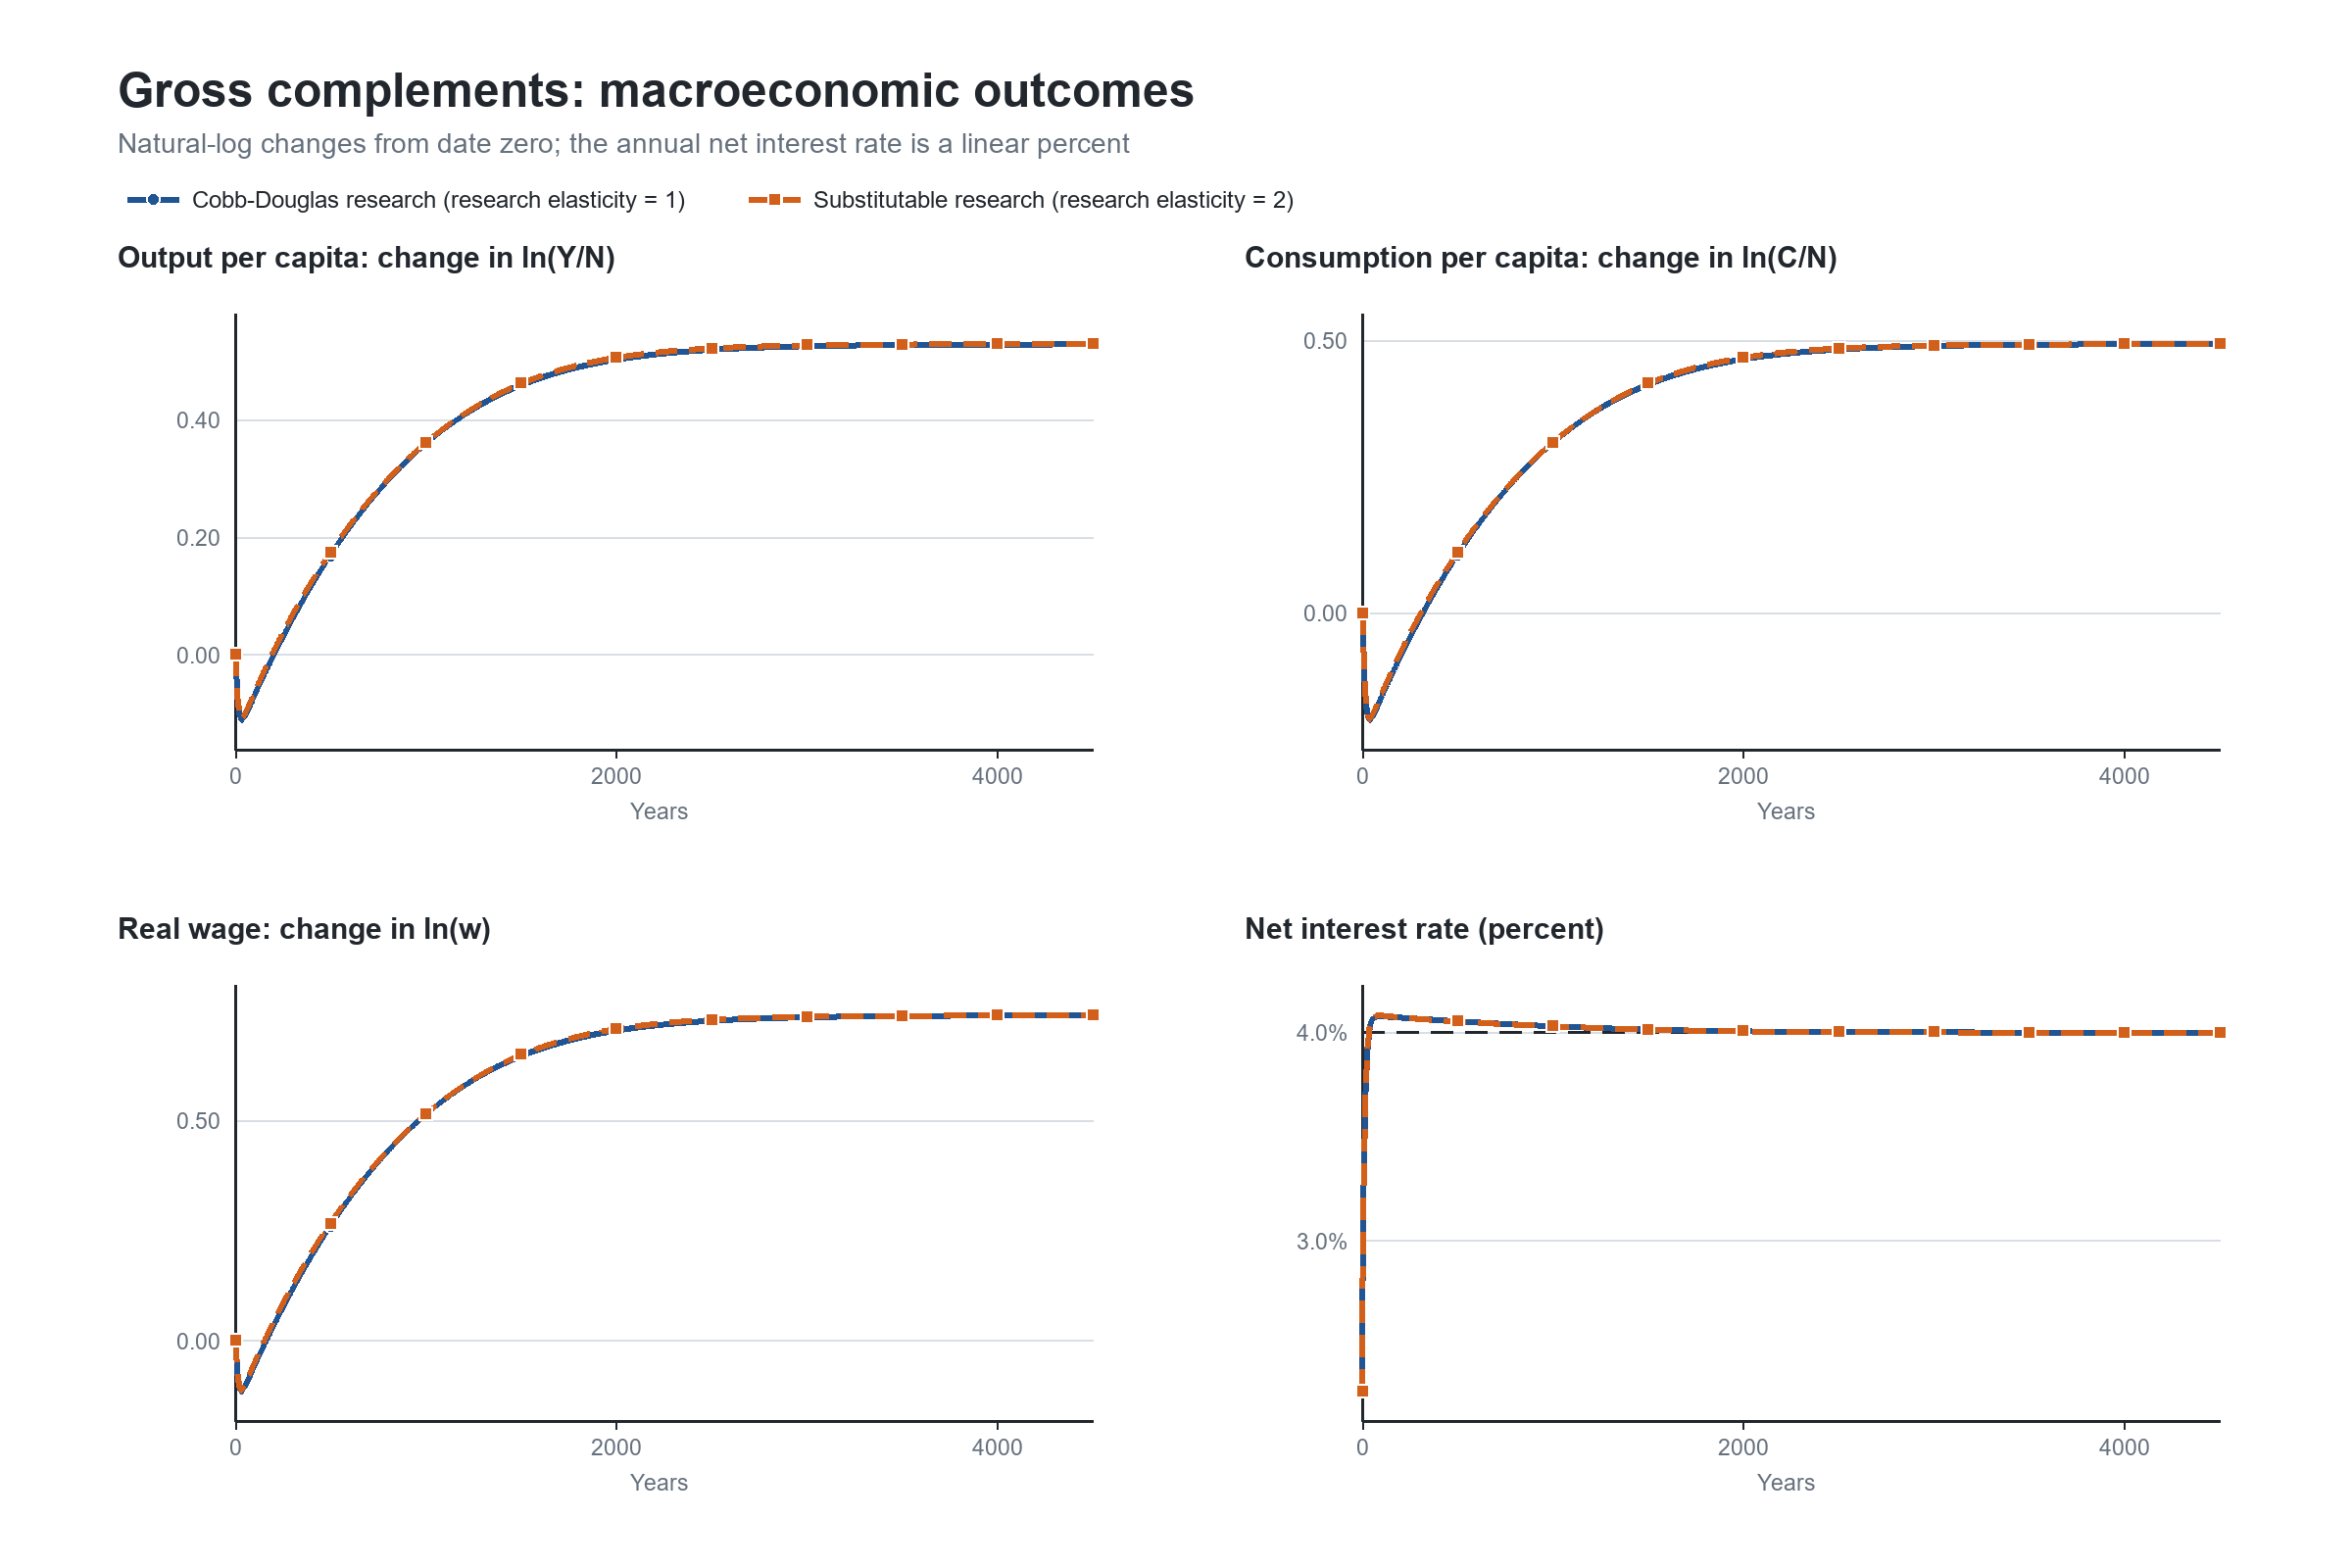
\includegraphics[width=\textwidth]{figures_axm/axm_complements_macro_prices.png}
\caption{Macroeconomic transition with \(\sigma_{XL}=0.75\). The first three
panels show natural-log changes from date zero; the last shows the annual net
interest rate. Blue solid lines use \(\sigma_{HM}=1\), and orange dashed lines
use \(\sigma_{HM}=2\). Model time is a numerical normalization, not a dated
forecast.}
\label{fig:axm-complement-macro}
\end{figure}

Figure \ref{fig:axm-complement-shares} shows the bottleneck directly. Production
labor approaches the population, \(X/(AL)\) approaches a finite ratio, inference
compute vanishes relative to output, and labor retains a positive income share.

\begin{figure}[H]
\centering
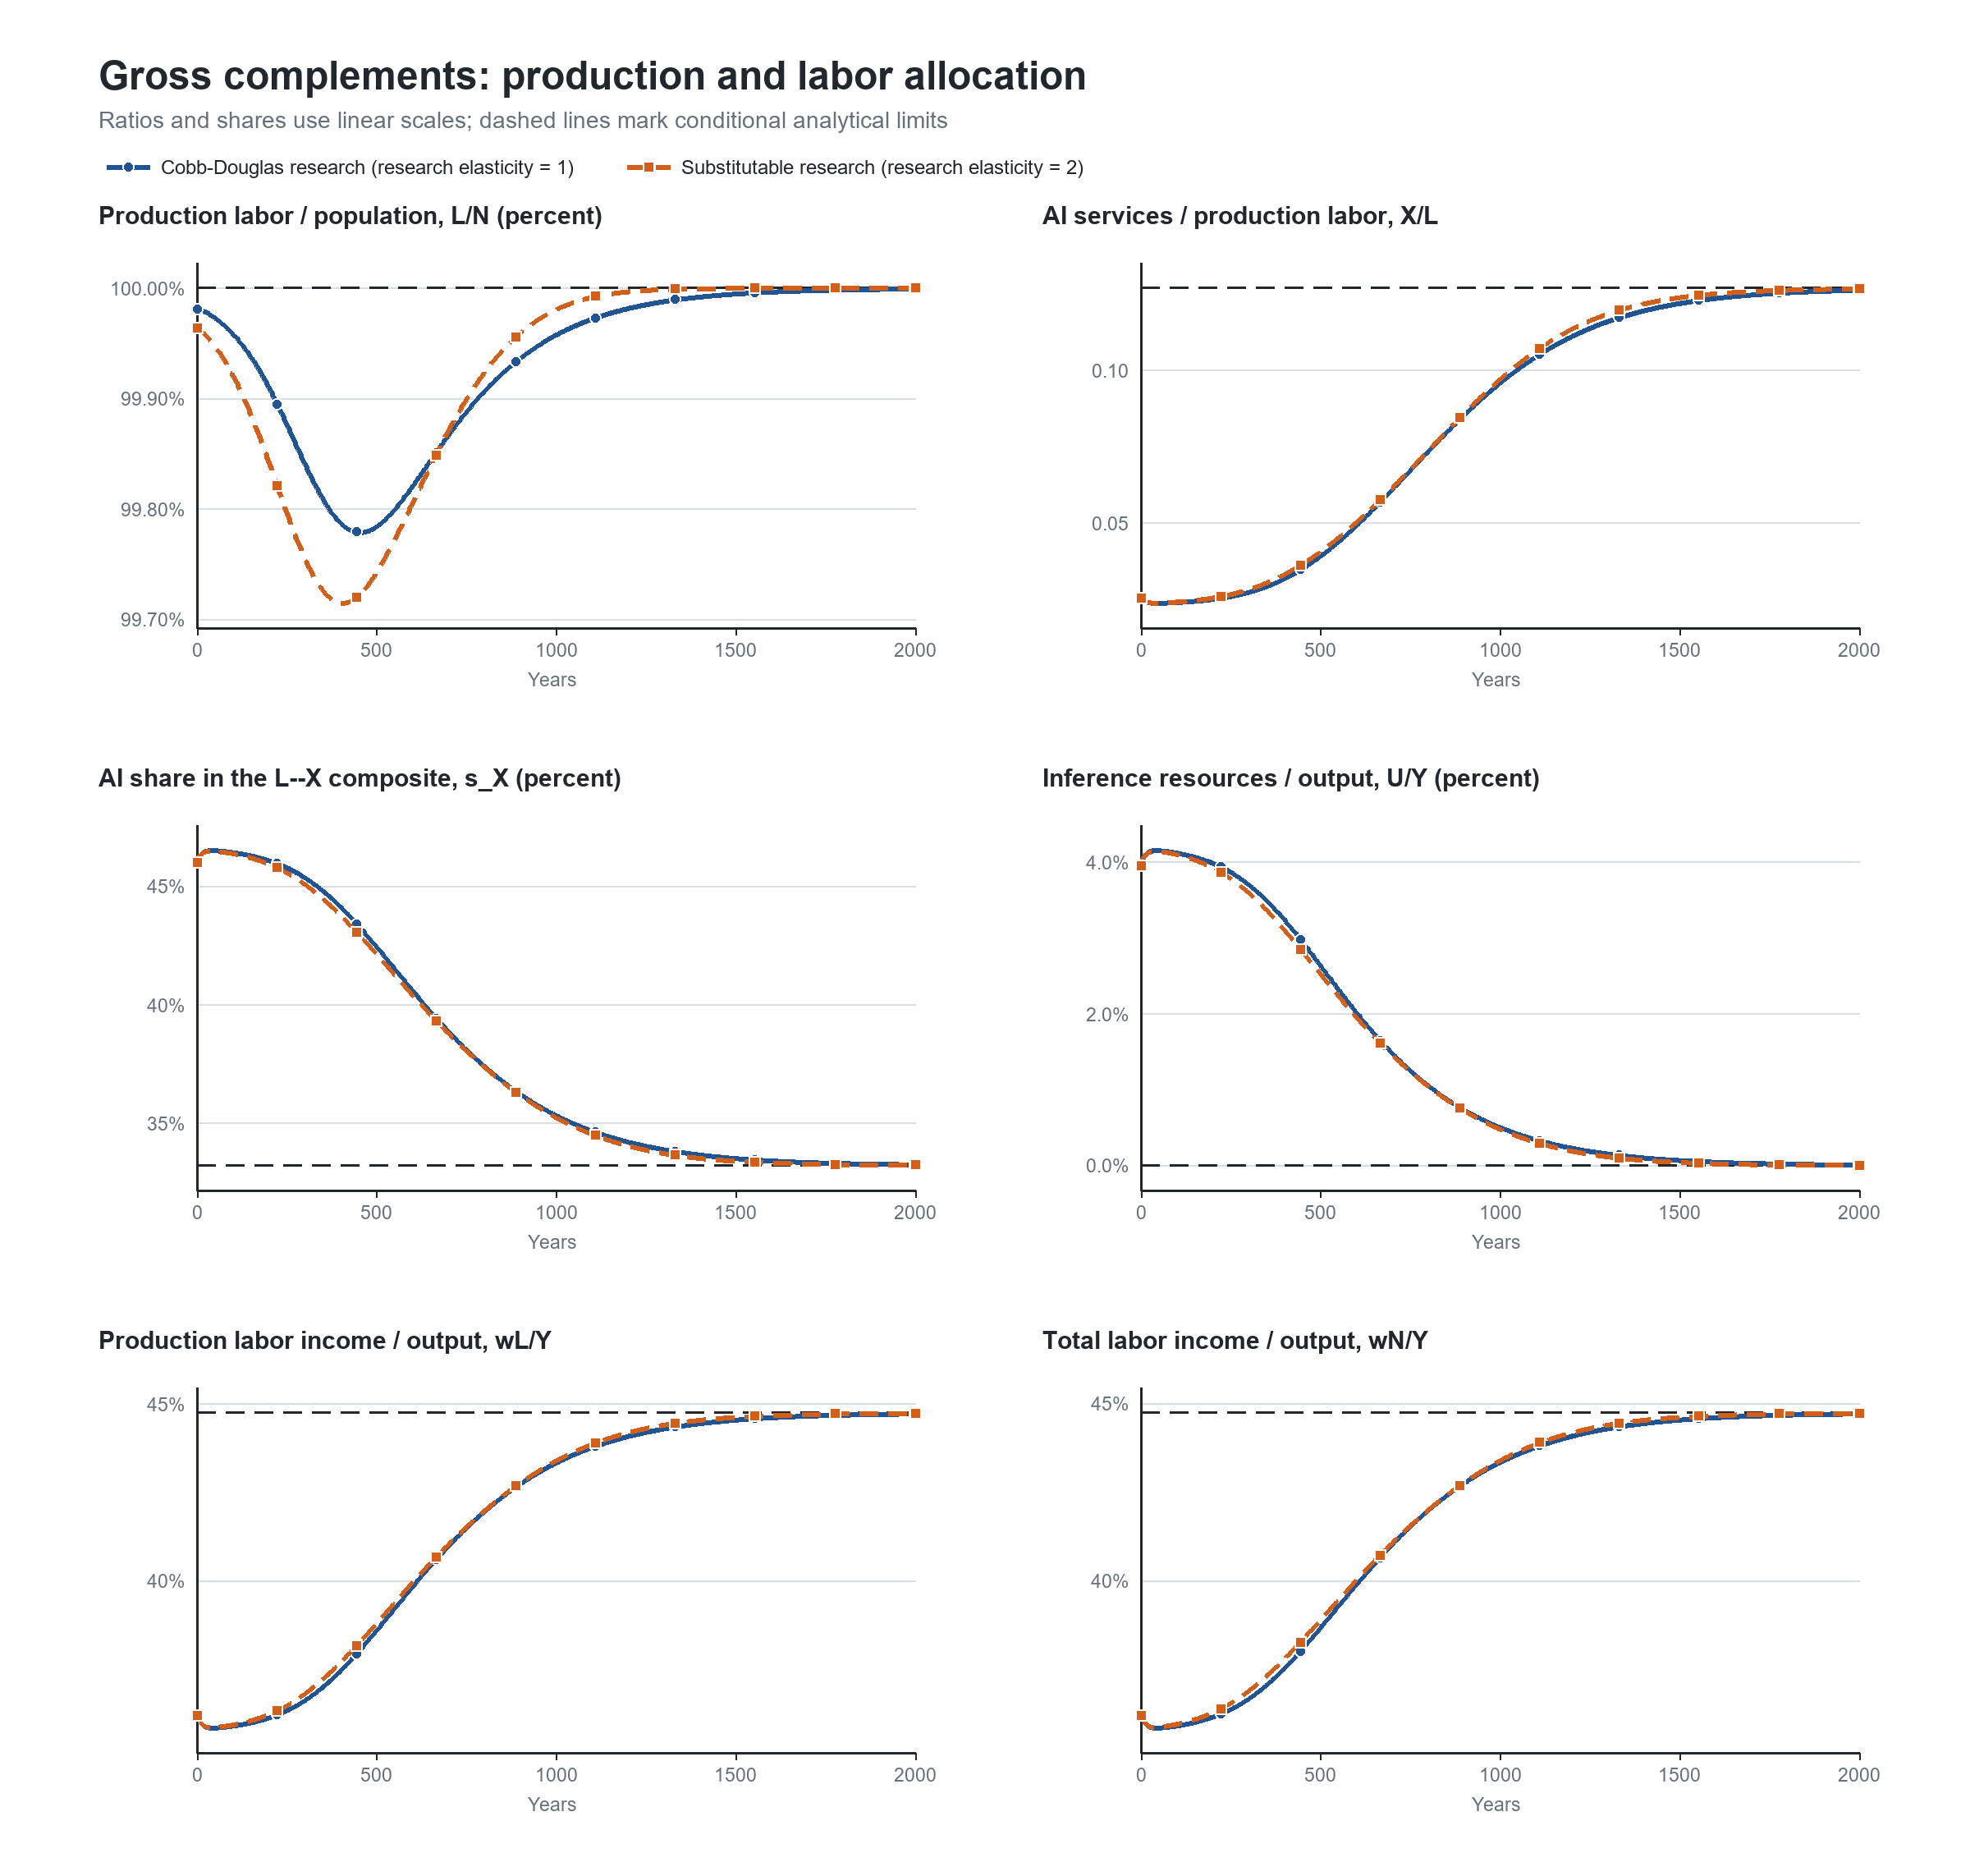
\includegraphics[width=\textwidth]{figures_axm/axm_complements_factor_shares_automation.png}
\caption{Production and labor allocation with \(\sigma_{XL}=0.75\). Here
\(s_X\) is AI production services' technological share within the labor--AI composite, not
their final-output income share. Ratios and shares use linear scales; the
\(L/N\) panel uses a focused vertical scale. Horizontal reference lines are
conditional analytical limits.}
\label{fig:axm-complement-shares}
\end{figure}

Figure \ref{fig:axm-complement-research} shows that research can still become
almost fully automated. With substitutable research inputs, \(s_M\) approaches
one and \(H/N\) approaches zero, while capability continues to rise.

\begin{figure}[H]
\centering
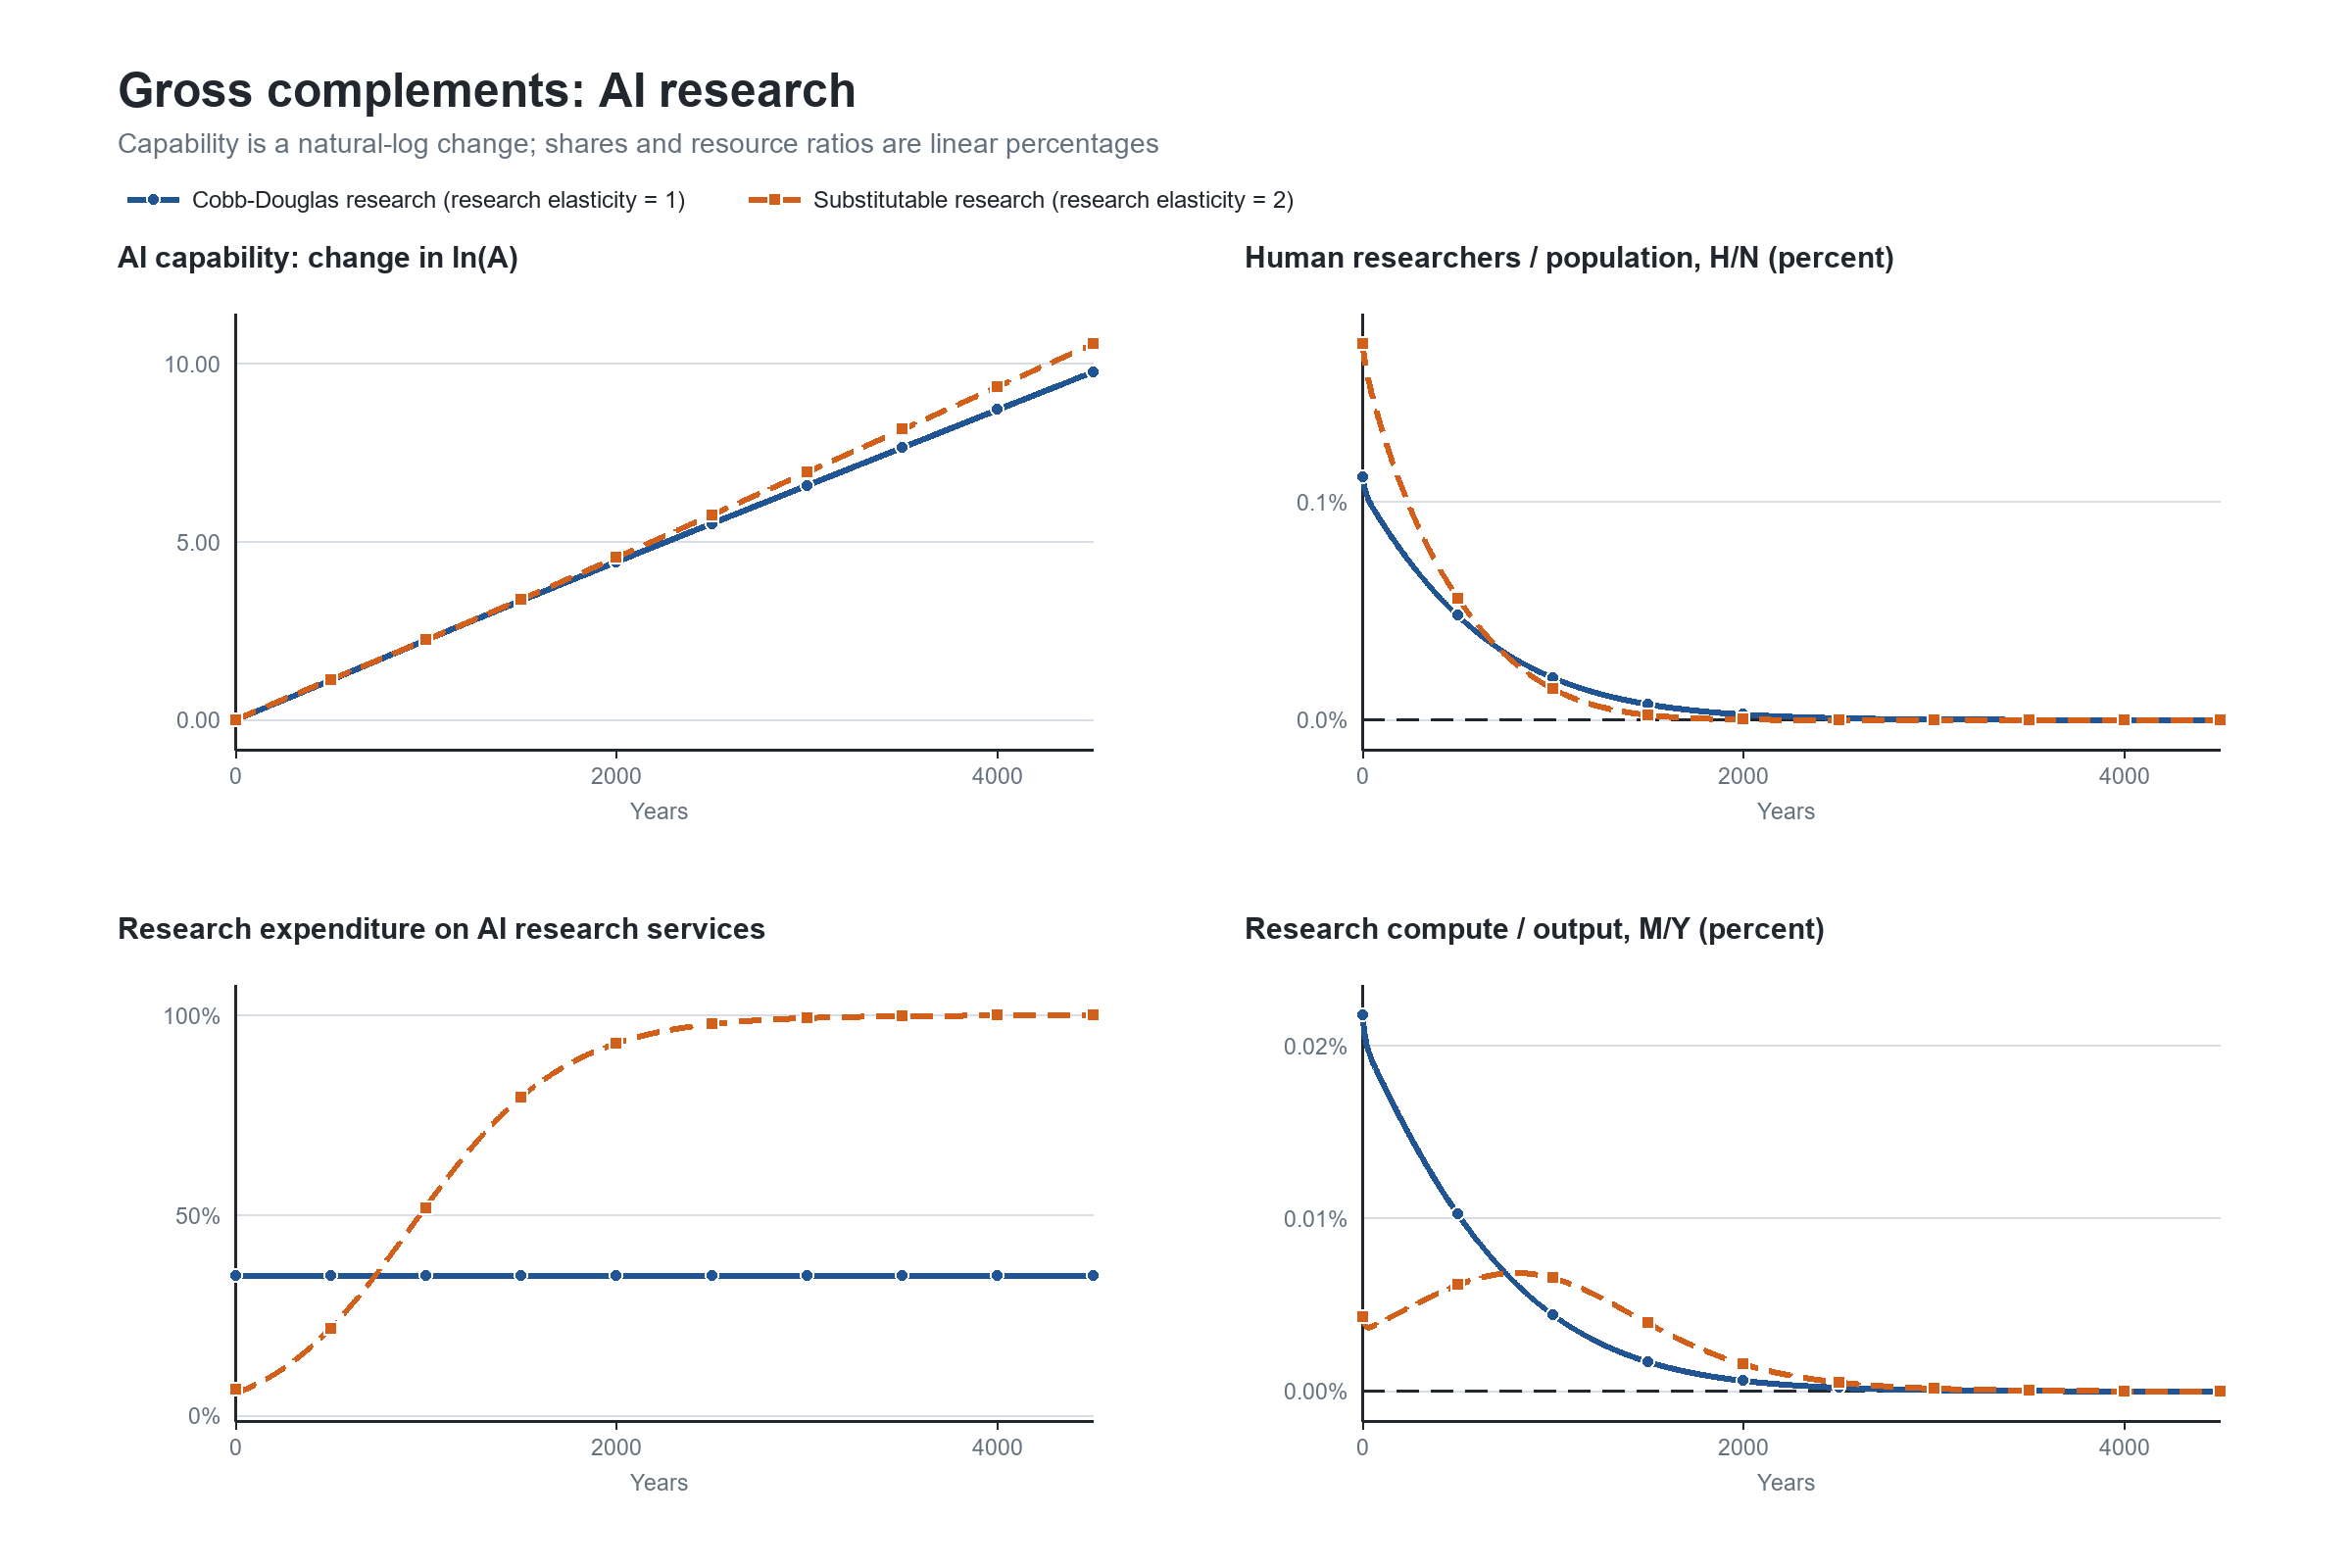
\includegraphics[width=\textwidth]{figures_axm/axm_complements_research_resources.png}
\caption{AI research with \(\sigma_{XL}=0.75\). Capability is shown as a
natural-log change from date zero. The human-research population share, the
share of research expenditure allocated to AI research services, and research compute relative to output
are percentages on linear scales. Positive allocations at every saved finite
date preserve interiority even as \(H/N\) and \(M/Y\) approach zero.}
\label{fig:axm-complement-research}
\end{figure}

At the terminal date with substitutable research, \(s_M=0.99982\) and
\(H/N=1.8\times10^{-11}\), yet labor's aggregate income share approaches 0.4474.
Research automation therefore does not remove the production bottleneck.

\subsection{Cases II and III: unit elasticity in final production}

The two unit-elasticity cases share the same final-production reduction. They
differ in the research-input limit and are therefore presented with a common
analytical characterization followed by separate case implications and a joint
numerical comparison.

\subsubsection{Common analytical characterization}

Set \(\sigma_{XL}=1\), and define
\begin{equation}
 \beta=(1-\alpha)\omega_X,\qquad
 \lambda=(1-\alpha)\omega_L,\qquad
 \nu=\frac{\beta}{\lambda}=\frac{\omega_X}{\omega_L}.
 \label{eq:axm-cd-definitions}
\end{equation}
Combining the final-good firm's AI-demand condition, the monopolist's markup
condition, and market clearing for AI production services with \(X=BU\) gives
\begin{equation}
 \frac{U}{Y}=\beta^2,
 \label{eq:axm-inference-share-cd}
\end{equation}
Substituting that identity into final production gives the reduced equation
\begin{equation}
 Y^{1-\beta}
 =K^\alpha(AL)^\lambda(\beta^2B)^\beta.
 \label{eq:axm-reduced-cd}
\end{equation}
On a balanced path with constant \(K/Y\) and a positive constant \(L/N\), this
equation gives
\begin{equation}
 g_Y=n+\gamma_A+\nu g_B.
 \label{eq:axm-output-growth-cd}
\end{equation}

It is useful to treat Cobb--Douglas research and research that asymptotically relies on AI research services
separately. Let
\begin{equation}
 \bar s=
 \begin{cases}
  \omega_M,&\sigma_{HM}=1,\\
  1,&\sigma_{HM}>1\text{ and }Bw\to\infty.
 \end{cases}
 \label{eq:axm-sbar}
\end{equation}
Define the feedback denominator
\begin{equation}
 D(\bar s)=1-\eta\bar s(1+\nu).
 \label{eq:axm-feedback-denominator}
\end{equation}

\begin{proposition}[Balanced-growth candidates at unit elasticity]
\label{prop:axm-cd-bgp}
Suppose \(\sigma_{XL}=1\), research remains interior, total research expenditure
\((wH+M)/Y\) converges to a positive output share, and \(K/Y\), \(C/Y\), and
\(L/N\) converge to positive constants. Suppose also that \(g_B\) converges to a
positive constant regularly, in the sense that \(\dot g_B/g_B\to0\).

\begin{enumerate}[label=(\roman*)]
\item If \(\sigma_{HM}=1\), every such balanced-growth equilibrium must have
 \(D(\omega_M)>0\).
\item If \(\sigma_{HM}>1\), the balanced-growth restrictions imply
 \(Bw\to\infty\) and \(s_M\to1\); every such equilibrium must have \(D(1)>0\).
\end{enumerate}

If the relevant denominator is positive, the only growth rates consistent with
these necessary restrictions are
\begin{equation}
 g_B=\frac{\eta(n+\bar s\gamma_A)}{D(\bar s)},\qquad
 g_Y=g_K=g_C=n+\gamma_A+\nu g_B,\qquad
 g_w=\gamma_A+\nu g_B.
 \label{eq:axm-cd-growth-rates}
\end{equation}
The remaining prices and quantities have the candidate rates
\begin{align}
 g_U&=g_M=g_Y,&
 g_X&=g_Y+g_B,&
 g_{p_X}&=-g_B,\\
 g_q&=g_Y-g_B,&
 g_E&=\frac{g_B}{\eta},&
 g_L&=n.
 \label{eq:axm-cd-remaining-rates}
\end{align}
Human research satisfies
\begin{equation}
 g_H=
 \begin{cases}
 n,&\sigma_{HM}=1,\\
 n-(\sigma_{HM}-1)[\gamma_A+(1+\nu)g_B],
 &\sigma_{HM}>1,\ s_M\to1.
 \end{cases}
 \label{eq:axm-human-research-growth}
\end{equation}
Thus \(H/N\) converges to a positive constant in the Cobb--Douglas research
case, whereas it falls asymptotically at rate
\((\sigma_{HM}-1)[\gamma_A+(1+\nu)g_B]\) when research inputs are gross substitutes.
Let \(\gamma=\gamma_A+\nu g_B\). The candidate output shares are
\begin{align}
 u&\equiv\frac{U}{Y}=\beta^2,\\
 i&\equiv\frac{\dot K+\delta K}{Y}
 =\frac{\alpha(n+\gamma+\delta)}{\rho+\delta+\gamma},\\
 m&\equiv\frac{M}{Y}
 =\frac{\beta^2\eta\bar s\,g_B}
 {\rho-n+(1-\eta\bar s)g_B},\\
 c&\equiv\frac{C}{Y}=1-u-i-m.
 \label{eq:axm-cd-shares}
\end{align}
The denominator in \(m\) is positive under \(\rho>n\), \(0<\eta<1\), and
\(0<\bar s\leq1\).
The computed share \(c\) must coincide with the positive limit hypothesized above.
An interior equilibrium also requires the monopoly second-order condition and
nonnegative limiting values of \(L/N\) and \(H/N\) that sum to one. Under the
maintained restriction \(\rho>n\), the candidate also satisfies both
transversality conditions.
\end{proposition}

The proposition states necessary growth restrictions and lists the remaining
conditions needed for existence; it does not infer existence from \(D>0\) alone.

The Cobb--Douglas research case admits a stronger constructive result. Define
\begin{equation}
 \ell^*=\frac{\lambda\omega_M}
 {\lambda\omega_M+m^*\omega_H},
 \label{eq:axm-cd-human-labor-share}
\end{equation}
where \(m^*\) is the share in \eqref{eq:axm-cd-shares} evaluated at
\(\bar s=\omega_M\).

\begin{proposition}[Existence and local selection with Cobb--Douglas human research]
\label{prop:axm-cd-human-existence}
Suppose \(\sigma_{XL}=\sigma_{HM}=1\), \(D(\omega_M)>0\),
\(\beta\leq1/2\), \(\eta(1+\omega_M)\leq1\), \(\rho>n\), and the
shares in \eqref{eq:axm-cd-shares} satisfy \(c^*>0\). Then, for every
\(A_0,N_0>0\), there are positive \(K_0,B_0,C_0,q_0\) and a regular interior
balanced-growth equilibrium with \(L/N=\ell^*\).

At the baseline calibration \(\gamma_A=0\), the normalized Jacobian has roots
\begin{equation}
 -0.08967,\qquad -0.002945,\qquad 0.03100,\qquad 0.12971.
 \label{eq:axm-cd-human-jacobian-roots}
\end{equation}
The projection of its stable eigenspace onto \((K,B)\) is nonsingular.
Consequently, consumption and the shadow value of capability are locally unique
functions of the two predetermined stocks, and the resulting nearby paths
converge to the balanced-growth equilibrium.
\end{proposition}

The result does not apply the automated benchmark's Jacobian to a model with
human research. The Appendix derives the human-research Jacobian from its own
labor-allocation and research equations. When \(\sigma_{HM}>1\), human research
vanishes only asymptotically; the corresponding finite-date Jacobian must be
computed from the interior static map.

\paragraph{Feedback-matrix interpretation.}
The feedback accounting of \citet{davidsonetal2026} makes the denominator
transparent. Let \(\widetilde g_Y=g_Y-(n+\gamma_A)\). The limiting balanced-growth
restrictions can be written as
\begin{equation}
 \begin{pmatrix}g_B\\ \widetilde g_Y\end{pmatrix}
 =
 \begin{pmatrix}\eta(n+\bar s\gamma_A)\\0\end{pmatrix}
 +
 \underbrace{\begin{pmatrix}
  \eta\bar s&\eta\bar s\\
  \nu&0
 \end{pmatrix}}_{\mathcal F(\bar s)}
 \begin{pmatrix}g_B\\ \widetilde g_Y\end{pmatrix}.
 \label{eq:axm-feedback-matrix}
\end{equation}
The upper-left entry is the technological loop
\(B\to BM\to\dot B\). The off-diagonal cycle is the economic loop
\(B\to Y\to M\to BM\to\dot B\). Consequently,
\begin{equation}
 \det[I-\mathcal F(\bar s)]
 =1-\eta\bar s(1+\nu)=D(\bar s),
 \qquad
 r_{\mathrm{sp}}(\mathcal F)
 =\frac{\eta\bar s+
 \sqrt{(\eta\bar s)^2+4\eta\bar s\nu}}{2}.
 \label{eq:axm-feedback-radius}
\end{equation}
Here \(r_{\mathrm{sp}}\) denotes the spectral radius; this notation avoids
confusing it with the household discount rate \(\rho\). Because \(\mathcal F\)
is nonnegative, \(r_{\mathrm{sp}}(\mathcal F)<1\) if and only if
\(D(\bar s)>0\). In that case,
\[
 \begin{pmatrix}g_B\\ \widetilde g_Y\end{pmatrix}
 =[I-\mathcal F(\bar s)]^{-1}
 \begin{pmatrix}\eta(n+\bar s\gamma_A)\\0\end{pmatrix}.
\]
Thus \(1/D(\bar s)\) is the scalar feedback multiplier after eliminating
\(\widetilde g_Y\), analogous to the relevant element of Davidson et al.'s
Leontief inverse.

Exogenous labor-productivity growth changes the source vector through
\(n+\bar s\gamma_A\), but it does not change the feedback matrix or its
stability threshold.

Equivalently, the reduced technological and economic gains are
\[
 G_T=\eta\bar s,\qquad
 G_E=\eta\bar s\nu,\qquad
 D=1-G_T-G_E.
\]
Table \ref{tab:axm-feedback-accounting} applies this decomposition to the two
unit-elasticity benchmarks. Research substitution raises the total gain from
0.0875 to 0.2500 and the feedback multiplier from 1.096 to 1.333. Even
\(\bar s=1\) remains below the critical value:
\(\bar s_{\mathrm{crit}}=[\eta(1+\nu)]^{-1}=4>1\).

\begin{table}[H]
\centering
\small
\begin{tabular}{lrrrrrr}
\toprule
Research limit & \(\bar s\) & \(G_T\) & \(G_E\) & \(G_T+G_E\) & \(D\) & \(1/D\)\\
\midrule
\(\sigma_{HM}=1\) & 0.35 & 0.0700 & 0.0175 & 0.0875 & 0.9125 & 1.096\\
\(\sigma_{HM}>1,\ s_M\to1\) & 1.00 & 0.2000 & 0.0500 & 0.2500 & 0.7500 & 1.333\\
\bottomrule
\end{tabular}
\caption{Davidson-style feedback accounting for the unit-elasticity benchmark
\citep{davidsonetal2026}. The reduced scalar gain is \(G_T+G_E\).
These are balanced-growth diagnostics, not calibrated probabilities or task
shares.}
\label{tab:axm-feedback-accounting}
\end{table}

This mapping also marks the boundary of what can be imported. Davidson et al.'s
spectral-radius theorem classifies a positive monomial system; their macroeconomic
application obtains such a system under fixed saving and resource-allocation
shares. Here \(D\leq0\) rules out the finite positive
balanced-growth candidate, but does not by itself prove double-exponential growth
or a finite-time singularity. Such a conclusion must also determine prices,
allocations, the developer's costate, and the transversality conditions.

\subsubsection{Adoption from the no-AI balanced-growth path}
\label{sec:axm-ai-adoption-experiment}

I first compare the automated-research benchmark with its no-AI counterfactual.
Before date zero, the economy is on the Ramsey--Cass--Koopmans balanced-growth
path with \(\omega_X=0\). At date zero, \(\omega_X\) increases to 0.20 and
\(\sigma_{XL}=1\). Physical capital, labor productivity, and population are
predetermined, so \(K_0\), \(A_0\), and \(N_0\) are inherited from the no-AI
path.

The no-AI equilibrium does not determine \(B_0\), because capability does not
affect any allocation when \(\omega_X=0\). I therefore calibrate the capability
available at adoption by requiring
\begin{equation}
 Y(0^+;\omega_X=0.20)=Y(0^-;\omega_X=0).
 \label{eq:axm-adoption-output-continuity}
\end{equation}
At unit elasticity, \eqref{eq:axm-inference-share-cd} and
\eqref{eq:axm-reduced-cd} imply that this condition is equivalent to
\(X_0=A_0L_0\). With \(A_0=N_0=L_0=1\), it gives
\begin{equation}
 B_0=\frac{1}{\beta^2Y_0^{\mathrm{RCK}}}=30.9316.
 \label{eq:axm-adoption-initial-capability}
\end{equation}
This value is an adoption-threshold calibration. It is not an equilibrium
condition and does not follow from continuing the positive-AI model through
\(\omega_X=0\). Given \(K_0\) and \(B_0\), the boundary-value problem selects
the jump variables \(C(0^+)\) and \(q(0^+)\). The matching rule isolates the
change in income shares from a mechanical change in initial output, but it does
not identify \(B_0\) empirically. The timing results below are therefore
conditional on \eqref{eq:axm-adoption-output-continuity}. At unit elasticity,
the production-labor, gross-capital, and inference-compute shares are fixed by
the model and do not depend on this matching rule.

The calibration satisfies the restrictions in Proposition
\ref{prop:axm-benchmark-equilibrium-existence}. In particular,
\(\eta=0.20<\alpha=0.33\), \(\beta=0.134<1/2\), \(2\eta=0.40<1\),
\(\Delta=0.402>0\), and \(\rho=0.04>n=0.003\). Hence the positive-AI model
has the analytical balanced-growth equilibrium characterized there. Its
per-capita output growth rate is \(g_Y^*-n=1.0867\) percent and its net
interest rate is \(r^*=5.0867\) percent. The adoption experiment starts far
from that reference path: \(\xi_B(0)=4.2445\). Moreover, the slow stable root
of the normalized system is \(-0.003194\), whose local half-life is about 217
years. Convergence should therefore not be visible within a short simulation
window.

Figure \ref{fig:axm-ai-adoption-macro} compares the two equilibrium paths.
Output does not jump by construction. Consumption falls by 2.26 percent at
adoption, while the real wage falls by 20 percent. The wage falls because the
production-labor share decreases from \(1-\alpha=0.67\) to
\((1-\alpha)\omega_L=0.536\), even though initial output is unchanged. Output
per person subsequently remains close to the no-AI path: after 250 years it is
0.61 percent higher. The net interest rate rises from 5 percent to 5.0035
percent over the same interval---an increase of only 0.0035 percentage points.
Since \(r=\alpha Y/K-\delta\), output continuity and the inherited capital
stock keep the interest rate at 5 percent at adoption. Output then grows
slightly faster than capital, so \(Y/K\) and the interest rate rise slowly.
Panel D extends the interest-rate path to 3,000 years and shows its convergence
to the analytical value \(r^*=5.0867\) percent. Its longer horizontal axis is a
numerical convergence audit, not a calendar forecast.

\begin{figure}[H]
\centering
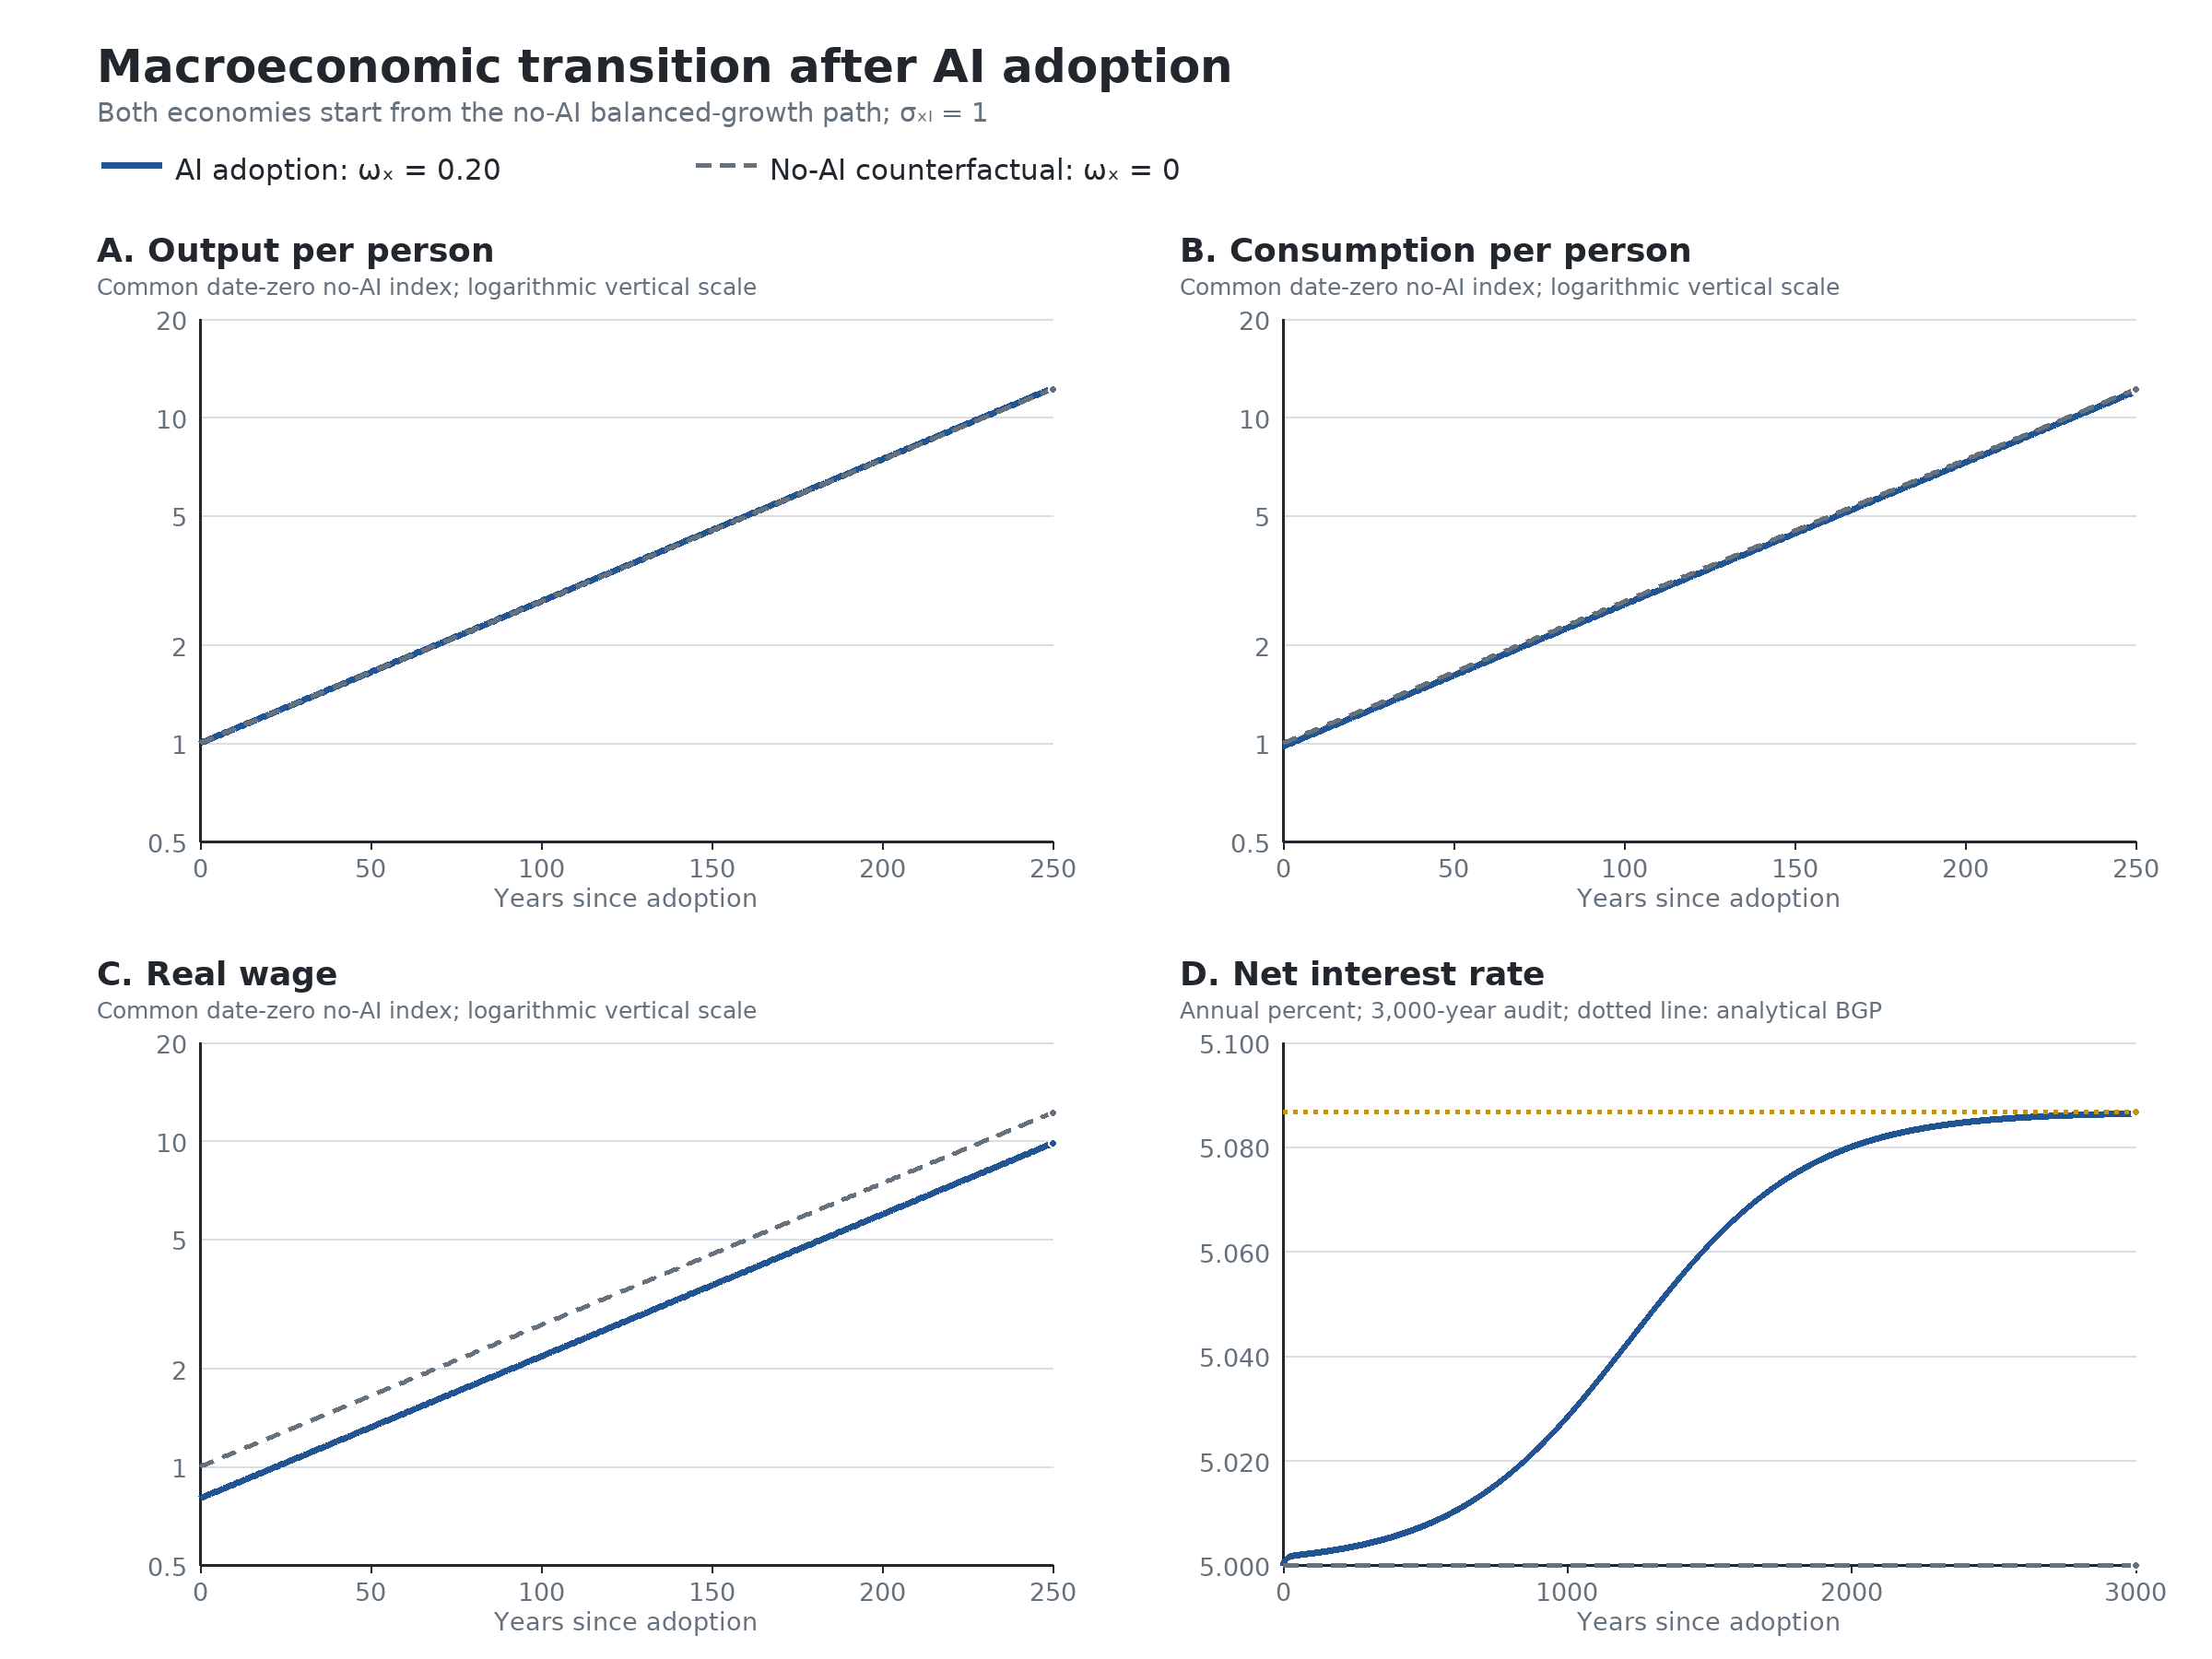
\includegraphics[width=\textwidth]{figures_axm/axm_ai_adoption_macro.png}
\caption{Macroeconomic effects of adopting AI production and autonomous AI
research at date zero. The AI path sets \(\omega_X=0.20\) and
\(\sigma_{XL}=1\); the counterfactual keeps \(\omega_X=0\). Output per person,
consumption per person, and the real wage use a common date-zero no-AI index
and logarithmic vertical scales over the first 250 years. The interest-rate
panel instead displays the full 3,000-year numerical audit; the dotted line is
the analytical balanced-growth value \(r^*=5.0867\) percent. Model time is not
a calendar forecast.}
\label{fig:axm-ai-adoption-macro}
\end{figure}

Figure \ref{fig:axm-ai-adoption-mechanism} explains why the macroeconomic
effects accumulate slowly. The annual growth rate of output per person rises
from 1.0006 percent at adoption to 1.0036 percent after 250 years, and
capability increases by 2.55 percent. The shadow value \(qB/Y\) changes little.
The numerical solution is extended to 3,000 years solely as a convergence
audit. Panel D of Figure \ref{fig:axm-ai-adoption-macro} displays the
interest-rate portion of that audit. At that horizon, per-capita growth is 1.08637 percent and the net
interest rate is 5.08637 percent, both within 0.00030 percentage points of
their analytical balanced-growth values. All other panels show the first 250
years.

\begin{figure}[H]
\centering
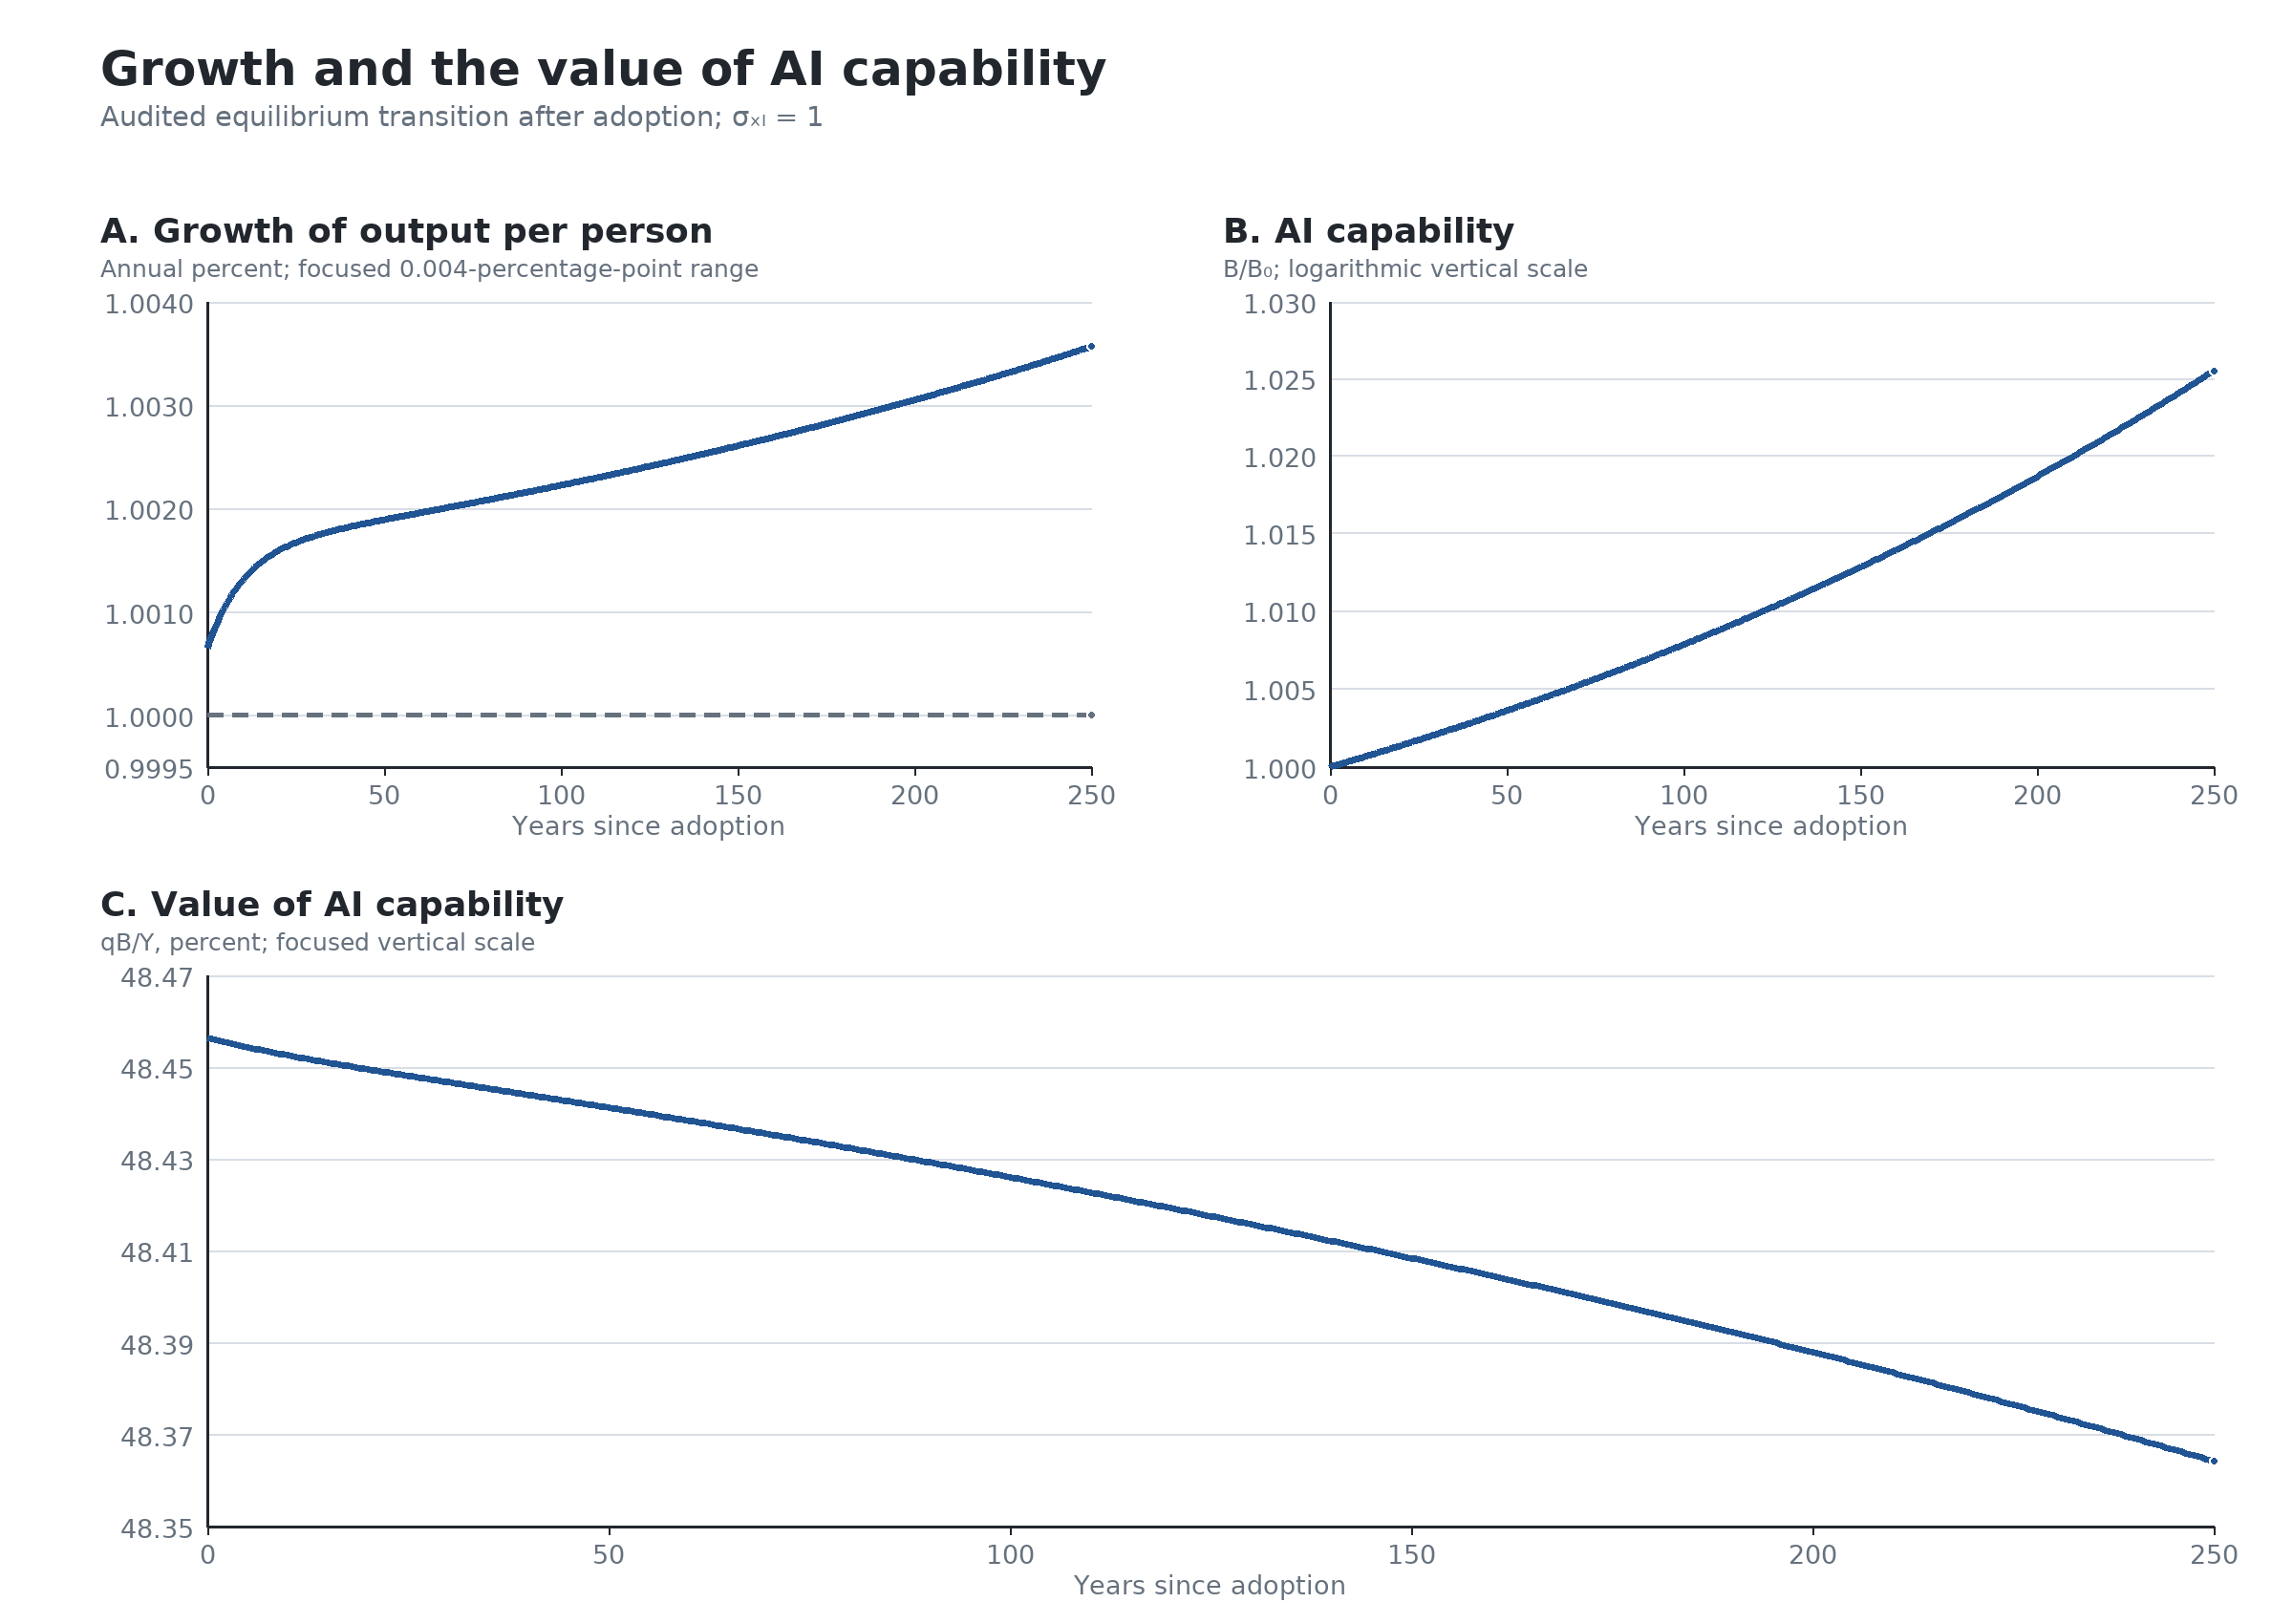
\includegraphics[width=\textwidth]{figures_axm/axm_ai_adoption_mechanism_distribution.png}
\caption{Growth and capability after AI adoption. Growth and \(qB/Y\) use
focused linear scales; the growth panel spans only 0.004 percentage points.
\(B/B_0\) uses a logarithmic scale. The gray dashed line in the first panel is
the no-AI growth rate.}
\label{fig:axm-ai-adoption-mechanism}
\end{figure}

Figure \ref{fig:axm-ai-adoption-distribution-paths} reports the five dated
components of the consolidated output decomposition. The distributional effect
is much larger than the growth effect and occurs immediately. At adoption,
labor's share falls from 67 percent in the no-AI counterfactual to 53.6 percent,
while the gross physical-capital share remains at 33 percent. Along the AI
path, \(wL/Y\), \((r+\delta)K/Y\), and \(U/Y\) remain constant. Over the first
250 years, \(M/Y\) rises from 0.00064 percent to 0.00141 percent of output, and
\(\Pi/Y\) falls by the same 0.00077 percentage points. Thus the large
redistribution occurs when AI enters production; the subsequent transition in
these shares is very small.

\begin{figure}[H]
\centering
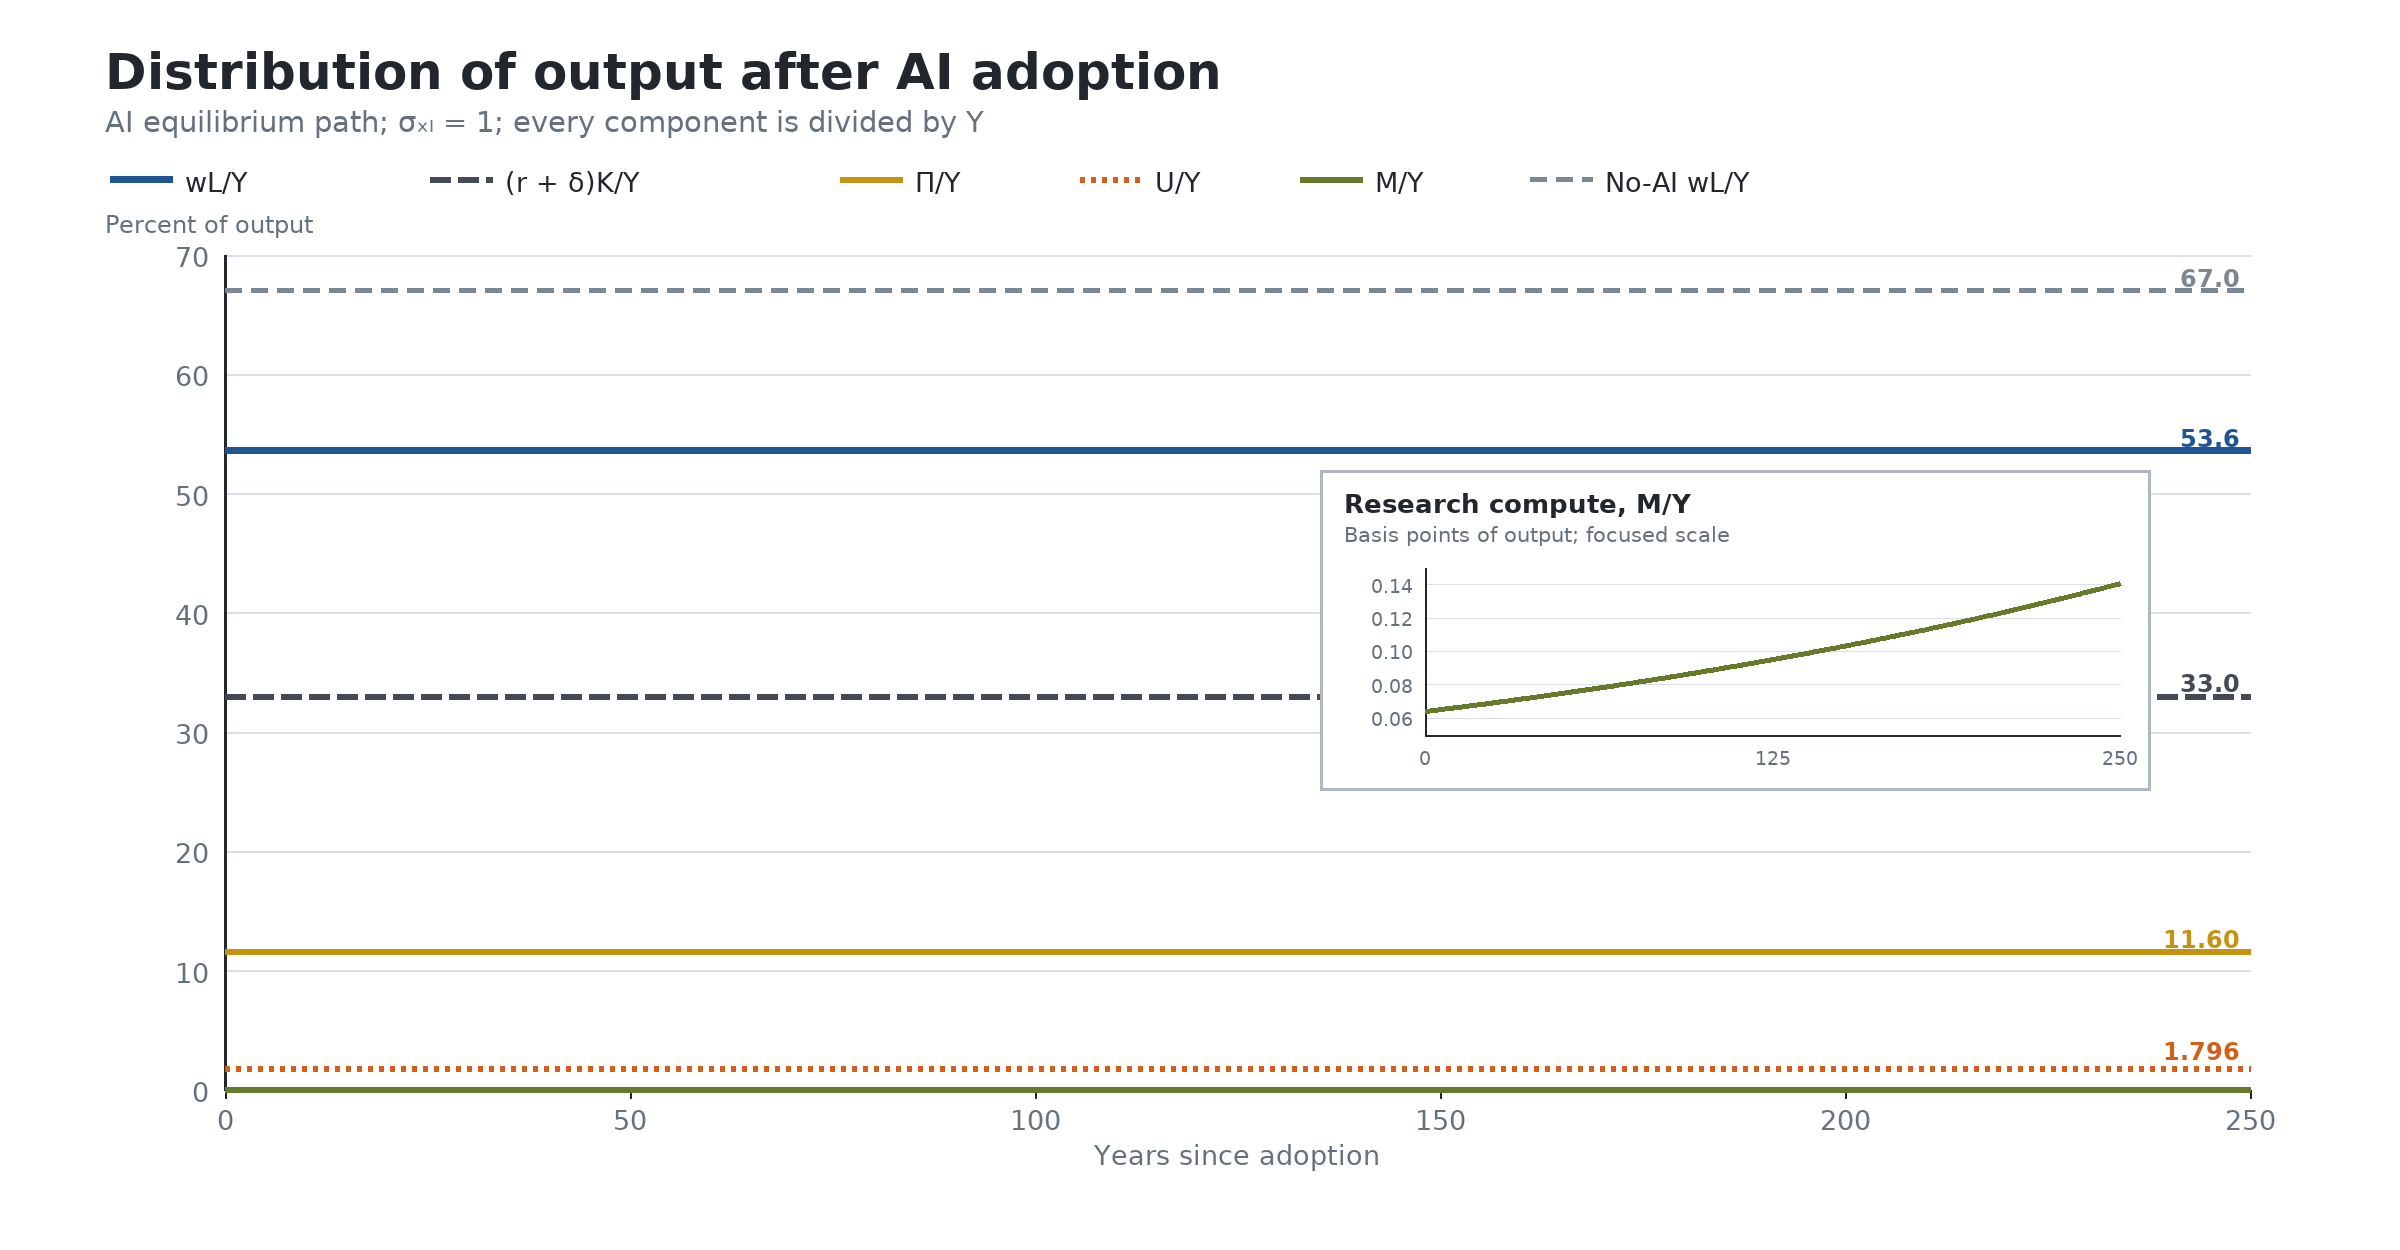
\includegraphics[width=\textwidth]{figures_axm/axm_ai_adoption_income_shares.png}
\caption{Trajectories of the consolidated output decomposition after AI
adoption. Every AI component is divided by \(Y\), and the five components sum
to one at every date. The gray dashed line reports the no-AI labor share as a
reference. The main panel uses percentage points on a linear scale. The inset
shows the same \(M/Y\) trajectory in basis points because it is too small to
read on the common scale. Since \(U\) and \(M\) are resource costs, this is a
consolidated decomposition of output rather than a factor-income decomposition
alone.}
\label{fig:axm-ai-adoption-distribution-paths}
\end{figure}

\subsubsection{\texorpdfstring{Case II: human-essential research, \(\sigma_{HM}=1\)}{Case II: human-essential research, sigma HM = 1}}
\label{sec:axm-case-human-essential}

When \(\sigma_{XL}=\sigma_{HM}=1\), the limiting share of research expenditure
allocated to AI research services is \(\bar s=\omega_M\). A balanced-growth candidate
therefore requires \(D(\omega_M)>0\) and the remaining feasibility conditions in
Proposition \ref{prop:axm-cd-bgp}. Human research and population grow at the same
rate, so \(H/N\) converges to a positive constant. The quantity of AI
research services can nevertheless grow faster than human research; human input
remains essential even as its quantity becomes small relative to \(BM\).

\subsubsection{\texorpdfstring{Case III: substitutable research, \(\sigma_{HM}>1\)}{Case III: substitutable research, sigma HM > 1}}
\label{sec:axm-case-substitutable-research}

When \(\sigma_{XL}=1\), \(\sigma_{HM}>1\), and the relative-price condition in
Proposition \ref{prop:axm-research-automation} holds, \(s_M\to1\) and the relevant
feedback denominator is \(D(1)\). A balanced-growth candidate therefore requires
\(D(1)>0\) and the remaining feasibility conditions in Proposition
\ref{prop:axm-cd-bgp}. Relative to Case II, automation strengthens the feedback
from capability to research. Human research grows more slowly than population and
\(H/N\) tends to zero on the candidate path.

\subsubsection{Numerical status}

The existing finite-horizon calculations comparing \(\sigma_{HM}=1\) and
\(\sigma_{HM}=2\) satisfy the dated equations, but their audit does not
establish an admissible infinite-horizon continuation satisfying both
transversality conditions. I therefore do not report their trajectories. The
analytical balanced-growth equilibria and local saddle-path results above remain
valid. A transition figure will be added only after the algorithm passes the
same equilibrium-admission test used for the benchmark paths.

\subsection{\texorpdfstring{Case IV: gross substitution in final production, \(\sigma_{XL}>1\)}{Case IV: gross substitution in final production, sigma XL > 1}}
\label{sec:axm-case-gross-substitution}

\subsubsection{Analytical characterization}

Let
\begin{equation}
 \theta=\frac{1-\alpha}{\alpha}.
 \label{eq:axm-theta}
\end{equation}
For \(\sigma_{XL}>1\), the static equilibrium conditions imply the exact
identity
\begin{equation}
 \frac{Y}{K}=B^\theta
 \left[
  (1-\alpha)s_X(1-e_X)
  \left(\frac{\omega_X}{s_X}\right)^{
   \sigma_{XL}/(\sigma_{XL}-1)}
 \right]^\theta.
 \label{eq:axm-high-sigma-exact-z}
\end{equation}
The expression in square brackets is continuous and strictly positive for
\(s_X\in(0,1]\), and it diverges as \(s_X\downarrow0\). It therefore has a
strictly positive lower bound. Hence \(B\to\infty\) implies
\(Y/K\to\infty\) even before establishing that AI production services dominate
the CES aggregate.

Along an interior branch on which \(s_X\to1\), AI production services do
eventually dominate that aggregate. Combining the same static conditions gives
\begin{equation}
 \frac{U}{Y}\to(1-\alpha)^2,\qquad
 \frac{Y}{K}\sim \mathcal D B^\theta
 \label{eq:axm-high-sigma-scaling}
\end{equation}
for a positive constant \(\mathcal D\).

\subsubsection{Finite-cap equilibrium regularization}
\label{sec:axm-finite-cap-gross-substitutes}

I now apply the finite-cap construction in Section
\ref{sec:axm-finite-cap-regularization}. The purpose is to replace the
finite-time boundary by an infinite-horizon economy for each
\(\overline B<\infty\), characterize that economy's terminal regime, and then
examine whether those equilibria have a meaningful limit as
\(\overline B\to\infty\).

For \(\sigma_{XL}>1\), define
\begin{equation}
 \mathcal D_\sigma=
 \left[(1-\alpha)^2
 \omega_X^{\sigma_{XL}/(\sigma_{XL}-1)}\right]^\theta,
 \qquad
 z_A(\overline B)=\mathcal D_\sigma\overline B^\theta,
 \label{eq:axm-capped-ai-only-productivity}
\end{equation}
where \(z_A(\overline B)\) is the limiting output--capital ratio when AI
production services dominate and capability is fixed at the frontier. Recall
\(\mathcal R=(\rho+\gamma_A+\delta)/\alpha\). The critical frontier is
\begin{equation}
 \overline B_c=
 \left(\frac{\mathcal R}{\mathcal D_\sigma}\right)^{1/\theta}.
 \label{eq:axm-critical-capability-frontier}
\end{equation}

To state the result, let
\begin{equation}
 \mathcal H_\sigma(s)=
 \left[
  (1-\alpha)s
  \left(1-\frac{1-s}{\sigma_{XL}}-\alpha s\right)
  \left(\frac{\omega_X}{s}\right)^{
   \sigma_{XL}/(\sigma_{XL}-1)}
 \right]^\theta.
 \label{eq:axm-capped-share-map}
\end{equation}
Equation \eqref{eq:axm-high-sigma-exact-z} is
\(Y/K=B^\theta\mathcal H_\sigma(s_X)\). The function
\(\mathcal H_\sigma\) is strictly decreasing on \((0,1]\), diverges as
\(s\downarrow0\), and satisfies
\(\mathcal H_\sigma(1)=\mathcal D_\sigma\).

\begin{proposition}[Terminal regimes of the finite-cap economy]
\label{prop:axm-capped-terminal-regimes}
Suppose \(\sigma_{XL}>1\), \(n+\gamma_A>0\), and \(\rho>n\). Consider a
regular finite-cap benchmark equilibrium that approaches
\(B=\overline B\), has convergent terminal ratios and growth rates, and has a
positive limiting consumption--output ratio.

If \(\overline B<\overline B_c\), the terminal regime is labor supported.
There is a unique \(\bar s_X\in(0,1)\) satisfying
\begin{equation}
 \mathcal R=\overline B^\theta\mathcal H_\sigma(\bar s_X).
 \label{eq:axm-capped-labor-supported-share}
\end{equation}
The limiting net interest rate and aggregate growth rate are
\begin{equation}
 \bar r=\rho+\gamma_A,\qquad
 \bar g=n+\gamma_A,\qquad
 \frac{wL}{Y}\to(1-\alpha)(1-\bar s_X)>0.
 \label{eq:axm-capped-labor-supported-rates}
\end{equation}

If \(\overline B>\overline B_c\), capital and AI production services outgrow
effective labor. The terminal regime is AI dominated and
\begin{align}
 \frac{Y}{K}&\to z_A(\overline B),&
 \bar r&=\alpha z_A(\overline B)-\delta,&
 \bar g&=n+\bar r-\rho>n+\gamma_A,
 \label{eq:axm-capped-ai-growth}\\
 \frac{wL}{Y}&\to0,&
 \frac{U}{Y}&\to(1-\alpha)^2,&
 \frac{p_XX}{Y}&\to1-\alpha.
 \label{eq:axm-capped-ai-shares}
\end{align}
The knife-edge \(\overline B=\overline B_c\) separates the two normalizations
and is not covered by the local terminal characterization.
\end{proposition}

The finite frontier therefore does not necessarily restore a positive labor
income share. It removes finite-time divergence, but a sufficiently high
frontier produces a finite-rate \(AK\)-type terminal regime in which labor
becomes asymptotically negligible. The rate is finite for every fixed
\(\overline B\), rather than uniformly bounded across frontiers.

\begin{proposition}[Research along a regular frontier approach]
\label{prop:axm-capped-frontier-research}
Maintain the conditions of Proposition
\ref{prop:axm-capped-terminal-regimes}. Suppose also that research compute and
the shadow value relative to output have positive finite limits and that the
frontier approach is regular. Let \(\bar g\) denote the terminal aggregate
growth rate in the relevant regime. Then
\begin{align}
 \frac{\dot B}{\overline B-B}&\to\bar g,&
 M&\to\overline M(\overline B)
 =\left[
  \frac{\bar g\,\overline B^{1-\eta}}{\chi}
 \right]^{1/\eta},
 \label{eq:axm-capped-terminal-research}\\
 g_q&\to\bar g,&
 \frac{X}{qB^2}&\to\bar r,&
 \frac{M}{Y}&\to0.
 \label{eq:axm-capped-terminal-shadow-value}
\end{align}
Both transversality objects have asymptotic log growth \(n-\rho<0\).
\end{proposition}

Combining Proposition \ref{prop:axm-capped-frontier-research} with the
developer's profit identity and the resource constraint completes the
consolidated decomposition in the AI-dominated regime:
\begin{equation}
 \frac{\Pi}{Y}\to\alpha(1-\alpha),\qquad
 \frac{C}{Y}\to
 \alpha(1-\alpha)+\frac{\rho-n}{z_A(\overline B)}.
 \label{eq:axm-capped-ai-consolidated-shares}
\end{equation}

These propositions characterize terminal restrictions for a finite-cap
equilibrium; they do not turn a solution of the capped dated equations into an
equilibrium automatically. A reported transition must still satisfy Definition
\ref{def:axm-benchmark-equilibrium}, including agent optimality and both
transversality conditions. Proposition
\ref{prop:axm-capped-developer-sufficiency} supplies a checkable developer
sufficiency condition near the frontier.

\begin{proposition}[The infinite-frontier limit]
\label{prop:axm-infinite-frontier-limit}
Suppose \(\sigma_{XL}>1\). On every compact subset of the positive state
space, the finite-cap state law, research condition, and costate equation
converge in \(C^1\) to their uncapped counterparts as
\(\overline B\to\infty\). Consequently, consider a sequence of finite-cap
equilibria for which \(\overline B_j\to\infty\), the selected initial jump
variables \((C_{0,j},q_{0,j})\) converge to a positive finite pair, and the
paths remain in a common compact subset on \([0,T]\). Their restrictions to
\([0,T]\) converge to the uncapped canonical path with the limiting initial
values. This finite-window statement does not establish that the sequence of
finite-cap equilibria exists or that its limit satisfies the uncapped
infinite-horizon transversality conditions.

The terminal regimes do not have a finite-rate limit. Once
\(\overline B>\overline B_c\),
\begin{equation}
 \bar r(\overline B)
 =\alpha\mathcal D_\sigma\overline B^\theta-\delta,\qquad
 \bar g(\overline B)
 =n-\rho-\delta+\alpha\mathcal D_\sigma\overline B^\theta,
 \label{eq:axm-capped-diverging-rates}
\end{equation}
so both rates diverge as \(\overline B\to\infty\). Hence taking the frontier
to infinity on a fixed pre-singular window is not the same operation as first
following each finite-cap equilibrium to its long run and then taking
\(\overline B\to\infty\).
\end{proposition}

The finite cap is therefore an equilibrium regularization of the pre-singular
branch, not a proof that the uncapped economy has an infinite-horizon
equilibrium. If capped equilibria can be constructed from the paper's initial
stocks, their limit can justify uncapped allocations on every compact interval
strictly before the singular date. It cannot supply an allocation at or beyond
that date.

Proposition \ref{prop:axm-research-burst} explains why the baseline uses the
stronger curvature restriction \(\eta<\alpha\). For all positive CES
elasticities and on each fixed regular horizon, the restriction makes the
developer's objective coercive over all nonnegative research policies with
finite expenditure and gives a finite truncated value. For the gross-substitutes
case in both nests studied here, the fixed-duration deviation establishes the
converse unboundedness result when \(\eta>\alpha\); the boundary
\(\eta=\alpha\) is not fully characterized.
The proposition does not supply compactness, prove that the finite-horizon
supremum is attained, establish a global or infinite-horizon optimum, select a
particular branch, or provide an admissible continuation through a finite-time
singularity.

\begin{proposition}[No finite-rate balanced growth with gross substitution]
\label{prop:axm-no-bgp}
Suppose \(\sigma_{XL}>1\), \(B\to\infty\), and an interior path satisfies the
dated equilibrium conditions. Then there is no balanced-growth path with finite
constant growth rates. In particular, \(Y/K\to\infty\), so the marginal product
of capital, the net interest rate, and household consumption growth become
unbounded.
\end{proposition}

The proposition is a conditional nonexistence result. It does not prove that every
initial condition enters the assumed unbounded-capability branch: capability may
remain bounded, a globally admissible continuation may fail, or the
infinite-horizon problem may not admit an optimum. The next result characterizes
the accelerating branch when it exists.

The bounded-capability alternative can be restricted without assuming that
normalized quantities or growth rates converge.

\begin{proposition}[No bounded capability with a bounded return]
\label{prop:axm-no-bounded-capability-tail}
Suppose the automated-research benchmark applies,
\(\sigma_{XL}>1\), \(n+\gamma_A>0\), and \(0<\eta<1\). There is no regular
interior infinite-horizon candidate satisfying the dated benchmark conditions
with both \(\sup_{t\geq0}B_t<\infty\) and
\(\sup_{t\geq0}r_t<\infty\).
\end{proposition}

\begin{proof}
Let \(\mathcal L=AN\) and \(G=n+\gamma_A>0\). Because capability is
nondecreasing, bounded capability implies
\(B_t\in[B_0,\bar B]\). Integrating its law gives
\begin{equation}
 B_t^{1-\eta}=B_0^{1-\eta}
 +(1-\eta)\chi\int_0^t M_s^\eta\dd s.
 \label{eq:axm-bounded-capability-integral}
\end{equation}
Hence \(\int_0^\infty M_t^\eta\dd t<\infty\). The research first-order
condition gives
\[
 M_t^\eta=(\chi\eta B_t^\eta)^{\eta/(1-\eta)}
 q_t^{\eta/(1-\eta)},
\]
so, because \(B_t\geq B_0>0\),
\begin{equation}
 \int_0^\infty q_t^{\eta/(1-\eta)}\dd t<\infty.
 \label{eq:axm-bounded-capability-q-integral}
\end{equation}

Now suppose \(r_t\leq\bar r\). The CES aggregate is bounded below by a
positive multiple of \(\mathcal L\). The capital-demand condition therefore
implies that \(K/\mathcal L\) is bounded away from zero. Homogeneity and the
unique static monopoly solution then give a uniform constant
\(\underline x>0\) such that
\(X_t/\mathcal L_t\geq\underline x\). In levels, the costate equation is
\[
 \dot q=a_tq-\frac{X}{B^2},\qquad
 a_t=r_t-\eta g_{B,t}\leq\bar r.
\]
Solving this linear equation backward from \(t+1\) to \(t\), using
\(q_{t+1}>0\), yields
\[
 q_t\geq\int_t^{t+1}
 e^{-\int_t^s a_v\dd v}\frac{X_s}{B_s^2}\dd s
 \geq c e^{Gt}
\]
for a constant \(c>0\). This contradicts
\eqref{eq:axm-bounded-capability-q-integral}. Therefore bounded capability and
a bounded return cannot coexist on such a candidate.
\end{proof}

The result is stronger than a stationary-limit argument, but it deliberately
leaves open a bounded-capability path with unbounded interest-rate spikes. The
next proposition records restrictions that every remaining irregular
continuation must satisfy.

\begin{proposition}[Necessary restrictions on an irregular gross-substitutes continuation]
\label{prop:axm-gross-substitutes-irregular-necessity}
Suppose the automated-research benchmark applies,
\(\sigma_{XL}>1\), \(n+\gamma_A>0\), and \(0<\eta<1\). Any regular interior
infinite-horizon equilibrium, if one exists, must satisfy one of the following:
\begin{enumerate}
 \item \(B\) is bounded and \(\sup_{t\geq0}r_t=\infty\); or
 \item \(B\to\infty\), and, writing \(z=Y/K\) and
 \(\theta=(1-\alpha)/\alpha\),
 \begin{equation}
  \liminf_{t\to\infty}\frac{g_{B,t}}{z_t}=0,
  \qquad
  \int_0^\infty e^{-(\rho-n)t}B_t^\theta\dd t<\infty.
  \label{eq:axm-irregular-necessary-restrictions}
 \end{equation}
\end{enumerate}
\end{proposition}

\begin{proof}
The first alternative follows from Proposition
\ref{prop:axm-no-bounded-capability-tail}. Suppose instead that \(B\to\infty\).
Equation \eqref{eq:axm-high-sigma-exact-z} gives
\(z_t\geq dB_t^\theta\) for some \(d>0\). If
\(\liminf g_B/z>0\), then eventually
\(\dot B=B g_B\geq\varepsilon dB^{1+\theta}\) for some
\(\varepsilon>0\), which makes \(B\) unbounded in finite time. An
infinite-horizon equilibrium must therefore satisfy the first restriction in
\eqref{eq:axm-irregular-necessary-restrictions}.

For the second, let \(c_h=C/N\). The household Euler equation gives
\[
 \log c_{h,t}=\log c_{h,0}-(\rho+\delta)t
 +\int_0^t(r_s+\delta)\dd s.
\]
Because \(r+\delta=\alpha z>0\), Tonelli's theorem shows that finiteness of the
household's improper utility integral requires
\[
 \int_0^\infty e^{-(\rho-n)t}(r_t+\delta)\dd t<\infty.
\]
Combining this condition with \(z_t\geq dB_t^\theta\) proves the second
restriction in \eqref{eq:axm-irregular-necessary-restrictions}.
\end{proof}

These restrictions do not assert that either irregular alternative exists.
They identify what a general nonexistence proof would still have to eliminate.
The next result characterizes the more regular unbounded AI-dominated
alternative.

\begin{conditionalresult}[AI-dominated singular limit]
\label{prop:axm-singular-limit}
Assume \(\sigma_{XL}>1\), \(0<\eta<\alpha<1\), and either the
automated-research benchmark or the human-research extension with
\(\sigma_{HM}>1\). Let an interior path satisfy all dated technology and service
identities, competitive price equations, static first- and second-order
conditions, market-clearing conditions, and canonical differential equations
on its maximal time interval. Suppose that the path approaches an AI-dominated
limit, with \(B\to\infty\) and \(s_X\to1\). In the human-research extension,
also suppose \(s_M\to1\); in the benchmark, set \(s_M\equiv1\). Suppose its
consumption, investment, and research-compute
shares---respectively \(C/Y\),
\((\dot K+\delta K)/Y\), and \(M/Y\)---as well as \(g_B/(Y/K)\) and \(qB/K\),
converge to positive finite limits.
Assume that the convergences of \(s_X\), \(s_M\), all the listed ratios, and the scaling ratio
\((Y/K)/(\mathcal D B^\theta)\to1\) are asymptotically regular: the growth rate
of each convergent ratio, divided by \(Y/K\), tends to zero. Write \(z=Y/K\) and
\[
 \Delta=1+\theta-\eta,\qquad
 h=\frac{\eta\alpha}{\Delta}.
\]
Then
\begin{align}
 \frac{g_B}{z}&\to h,&
 \frac{U}{Y}&\to(1-\alpha)^2,\\
 \frac{\dot K+\delta K}{Y}&\to\alpha-\theta h,&
 \frac{M}{Y}&\to\frac{\eta(1-\alpha)^2}{\Delta},\\
 \frac{qB}{K}&\to\frac{(1-\alpha)^2}{\eta\alpha},&
 \frac{C}{Y}&\to
 1-(1-\alpha)^2-\alpha+\theta h
 -\frac{\eta(1-\alpha)^2}{\Delta}.
 \label{eq:axm-singular-ratios}
\end{align}
Moreover,
\begin{equation}
 \dot z\sim\theta h z^2.
 \label{eq:axm-z-law}
\end{equation}
Because the limiting gross-investment share
\(\alpha-\theta h=\alpha(1-\eta)/(1-\alpha\eta)\) is positive, capital is
eventually increasing. Thus \(z\), and consequently output, become unbounded in
finite time.
For the wage result, define
\[
 \underline\sigma=
 \begin{cases}
  \sigma_{XL},&\text{in the automated-research benchmark},\\
  \min\{\sigma_{XL},\sigma_{HM}\},&\text{in the human-research extension}.
 \end{cases}
\]
In the human-research extension, the allocation of labor satisfies
\begin{equation}
 (H/N,L/N)\to
 \begin{cases}
  (1,0),&\sigma_{HM}<\sigma_{XL},\\
  (\bar h_N,1-\bar h_N),
      &\sigma_{HM}=\sigma_{XL}=\sigma,\\
  (0,1),&\sigma_{HM}>\sigma_{XL}.
 \end{cases}
 \label{eq:axm-singular-labor-allocation}
\end{equation}
In the equal-elasticity case, the limiting share is pinned down by
\begin{equation}
 \bar h_N=\frac{\mathcal R_\sigma}{1+\mathcal R_\sigma},\qquad
 \mathcal R_\sigma=\frac{\eta}{\Delta}A_*^{1-\sigma}
 \left[
  \frac{(1-\alpha)\omega_H\omega_X}{\omega_M\omega_L}
 \right]^{\sigma}.
 \label{eq:axm-singular-equal-elasticity-share}
\end{equation}
Here \(A_*=\lim_{t\uparrow T^*}A_t\) is finite and positive because labor
productivity grows exogenously and the singular date is finite.
In the benchmark, \(L=N\). In both versions, production labor income,
\(wL/Y\), and aggregate labor income, \(wN/Y\), vanish as shares of output,
while
\begin{equation}
 \frac{g_w}{z}\to
 \frac{\alpha-(\underline\sigma-1)h}{\underline\sigma}
 \label{eq:axm-wage-limit}
\end{equation}
which is positive if and only if
\(\underline\sigma<1/(\alpha\eta)\).
\end{conditionalresult}

\begin{proposition}[No regular benchmark continuation]
\label{prop:axm-no-regular-gross-substitutes-continuation}
Suppose the automated-research benchmark applies, \(\sigma_{XL}>1\),
\(0<\eta<\alpha<1\), and \(n+\gamma_A>0\). Consider a regular interior
candidate whose proposed long-run continuation belongs to either of the two
classes used by the algorithm:
\begin{enumerate}
 \item capability and the interest rate are bounded; or
 \item capability is unbounded and the conditions of Conditional Result
 \ref{prop:axm-singular-limit} hold.
\end{enumerate}
Neither continuation can complete the candidate as an admissible
infinite-horizon equilibrium.
\end{proposition}

\begin{proof}
The first continuation contradicts the developer's costate equation by
Proposition \ref{prop:axm-no-bounded-capability-tail}. Under the second,
Conditional Result \ref{prop:axm-singular-limit} gives
\(\dot z\sim\theta h z^2\), where \(z=Y/K\) and \(\theta h>0\). The maximal
path therefore ends at a finite singular date and is not defined for every
\(t\geq0\). Proposition \ref{prop:axm-no-zero-research-corner} also shows that
setting \(M=0\) at a finite date cannot rescue either continuation.
\end{proof}

Conditional Result \ref{prop:axm-singular-limit} characterizes a postulated
asymptotic branch of the model's necessary
conditions. Because the maximal interval ends at the singularity, it does not
establish existence or global optimality for the infinite-horizon problems, nor
does it establish that the branch is reached from arbitrary initial conditions.
Proposition \ref{prop:axm-no-regular-gross-substitutes-continuation} is an
exhaustion result only within the two regular terminal classes stated there. It
does not exclude either irregular alternative in Proposition
\ref{prop:axm-gross-substitutes-irregular-necessity}: bounded capability with
unbounded interest-rate spikes, or unbounded capability with
\(\liminf g_B/(Y/K)=0\) and sufficiently slow discounted growth. Nor does it
exclude another terminal regime not used by the algorithm.
Within that branch, workers move asymptotically toward the sector in which they
are harder to replace. The model delivers a sharp separation when
\(1<\underline\sigma<1/(\alpha\eta)\): aggregate labor income as a share of output
vanishes, but the wage eventually rises. Above the threshold, the same conditional
scaling implies an eventually falling wage. The case above the threshold should
not be interpreted without separately
checking monopoly optimality and convergence to the postulated branch.
At \(\underline\sigma=1/(\alpha\eta)\), the leading term in
\eqref{eq:axm-wage-limit} is zero, so this asymptotic calculation alone does not
determine the eventual direction of the wage.

The growth-rate transformation used by \citet{davidsonetal2026} provides a useful
interpretation of this conditional branch. The limiting ratios imply
\[
 \dot B\sim \kappa_B B^{\eta(1+\theta)}K^\eta,
 \qquad
 \dot K\sim \kappa_K B^\theta K
\]
for positive constants \(\kappa_B,\kappa_K\). Hence the growth rates satisfy
\begin{equation}
 \begin{pmatrix}
  \dot g_B/g_B\\[2pt] \dot g_K/g_K
 \end{pmatrix}
 \sim
 \underbrace{\begin{pmatrix}
  \eta(1+\theta)-1&\eta\\
  \theta&0
 \end{pmatrix}}_{\Omega_\infty}
 \begin{pmatrix}g_B\\g_K\end{pmatrix}.
 \label{eq:axm-singular-feedback-matrix}
\end{equation}
Under Assumption \ref{ass:axm-large-scale-curvature}, the diagonal
\(g_B\)-feedback coefficient is negative:
\[
 \eta(1+\theta)-1=\frac{\eta}{\alpha}-1<0.
\]
Nevertheless,
\[
 \det\Omega_\infty=-\eta\theta<0,
\]
so \(\Omega_\infty\) has one positive and one negative eigenvalue. The positive
eigenvalue is generated by the off-diagonal two-way link between capability
growth and capital growth. Making the diagonal feedback subcritical does not
eliminate the positive direction created by the coupled feedback system. This is
the matrix counterpart of \(\dot z\sim\theta h z^2\) on the postulated branch;
it does not establish global optimality, reachability, or an admissible
continuation beyond the finite-time boundary.

\subsubsection{Why no gross-substitutes trajectory is reported}

For \(\sigma_{XL}=1.01\), the algorithm follows the continuation order used on
the two sides of one: it starts from the exact strictly positive-AI
unit-elastic equilibrium, changes \(\sigma_{XL}\) on a short horizon, and then
extends the horizon while preserving the same dated equations and initial
stocks. The initial consumption and shadow-value jumps stabilize, but this does
not identify an infinite-horizon continuation. At \(T=5{,}000\), the terminal AI share
is only \(0.2303\), far from the AI-dominated limit. The local separation rate
\((\sigma_{XL}-1)\eta(n+\gamma_A)/\sigma_{XL}\) is
\(4.29\times10^{-5}\), whose inverse is about 23,300 model years. Near-unit
finite-window similarity is therefore expected even though the long-run
regimes differ.

Proposition \ref{prop:axm-no-bounded-capability-tail} rejects bounded
capability whenever the interest rate is bounded. The regular
AI-dominated alternative is the finite-time branch in Conditional Result
\ref{prop:axm-singular-limit}, not an infinite-horizon allocation. Proposition
\ref{prop:axm-gross-substitutes-concavity-gate} also shows that the sufficient
global concavity condition fails over the full counterfactual capability
domain at every date: its limiting service-capability elasticity is
\(1/\alpha=3.03>2\) under the calibration. For \(\sigma_{XL}=1.01\), optimized
operating profit first loses concavity at \(s_X=0.7386\), above the terminal
share in the finite-window calculation. Thus the saved segment remains on the
locally concave part of the state space, but the sufficient theorem cannot
compare it with all admissible alternatives. This failure is not a
nonexistence proof, but it prevents the computed first-order-condition branch
from being admitted as a globally optimal developer policy.

The older free-boundary calculation for
\((\sigma_{XL},\sigma_{HM})=(1.5,2)\) likewise solves the dated necessary
conditions only up to a finite artificial boundary. Under the equilibrium
definition in Section \ref{sec:axm-model}, neither calculation constructs an
admissible path for every \(t\geq0\). I therefore report no simulated
trajectory for \(\sigma_{XL}>1\). Both calculations remain in the repository
as diagnostics for the conditional analytical result, not as sources of paper
figures.

\subsection{Factor payments and resource uses across regimes}
\label{sec:axm-distributional-accounting}

The regimes can now be compared using the same accounting of factor payments
and resource uses. Zero profit in the final-good sector implies
\begin{equation}
 1=\frac{(r+\delta)K}{Y}+\frac{wL}{Y}+\frac{p_XX}{Y}
 =\alpha+(1-\alpha)(1-s_X)+(1-\alpha)s_X.
 \label{eq:axm-final-sector-distribution}
\end{equation}
Thus \(\alpha\) is the gross capital-payment share, including depreciation, and
\(s_X\) determines how the remaining output is divided between production labor
and purchases of AI production services.

Gross revenue from AI production services is not developer profit:
\begin{equation}
 \frac{p_XX}{Y}=\frac{U}{Y}+\frac{wH}{Y}+\frac{M}{Y}+\frac{\Pi}{Y}.
 \label{eq:axm-developer-revenue-distribution}
\end{equation}
Inference compute, research wages, and research compute are paid before the
residual \(\Pi\) is distributed. Substituting this identity into the final firm's
accounts yields the six-part decomposition in
\eqref{eq:axm-consolidated-distribution} without counting \(p_XX\) twice.

The final-production elasticity does not determine these shares by itself at a
finite date because \(s_X\) also depends on the equilibrium ratio \(X/(AL)\). The
propositions above determine the following conditional limiting shares. Under
complementarity, for any \(0<\sigma_{XL}<1\) satisfying the hypotheses of Propositions
\ref{prop:axm-complements} and \ref{prop:axm-complements-research},
\begin{equation}
 \frac{wN}{Y}\longrightarrow
 \frac{\sigma_{XL}(1-\alpha)^2}{1-\alpha\sigma_{XL}},
 \qquad
 \frac{p_XX}{Y},\frac{\Pi}{Y}\longrightarrow
 \frac{(1-\alpha)(1-\sigma_{XL})}{1-\alpha\sigma_{XL}}.
 \label{eq:axm-complement-distribution}
\end{equation}
At unit elasticity, \(s_X=\omega_X\), so the final-good firm's gross payment
shares are constant. On the conditional AI-dominated gross-substitutes branch,
\(s_X\to1\), aggregate labor income vanishes relative to output, and gross
revenue from AI production services approaches \(1-\alpha\).

Table \ref{tab:axm-distributional-synthesis} reports the conditional limits for
the three \(\sigma_{HM}=2\) benchmarks. The first two rows use balanced-growth
limits or candidates; the last uses the conditional pre-singular ratios.

\begin{table}[H]
\centering
\footnotesize
\setlength{\tabcolsep}{3.5pt}
\caption{Payments and resource uses at the conditional limits of the three benchmark regimes}
\label{tab:axm-distributional-synthesis}
\begin{tabular}{lrrrrrr}
\toprule
Final-production regime & \((r+\delta)K/Y\) & \(wL/Y\) & \(wH/Y\) & \(\Pi/Y\) & \(U/Y\) & \(M/Y\)\\
\midrule
Complements, \(\sigma_{XL}=0.75\) & 33.000 & 44.741 & 0.000 & 22.259 & 0.000 & 0.000\\
Unit elasticity, \(\sigma_{XL}=1\) & 33.000 & 53.600 & 0.000 & 11.567 & 1.796 & 0.038\\
Gross substitutes, \(\sigma_{XL}=1.5\) & 33.000 & 0.000 & 0.000 & 18.938 & 44.890 & 3.172\\
\bottomrule
\end{tabular}

\medskip
\parbox{0.95\textwidth}{\footnotesize \emph{Notes:} Entries are percentages of
\(Y\). The six components sum to final output without counting the intermediate
payment for AI production services twice. Zeros are limiting shares, not zero quantities at every
finite date. The first two rows are balanced-growth limits or candidates; the
last is the conditional pre-singular limit, not a proved infinite-horizon
equilibrium.}
\end{table}

The equilibrium transition figures above report this decomposition only for
paths that pass the equilibrium-admission audit. I do not combine them with the
gross-substitutes free-boundary calculation, because that calculation is not an
infinite-horizon equilibrium trajectory. The conditional last row of Table
\ref{tab:axm-distributional-synthesis} is therefore an analytical benchmark,
not a simulated income-distribution path.

The net interest rate and the capital-income share are also different objects.
The gross capital-payment share remains \(\alpha\) in every regime, but
\begin{equation}
 \frac{rK}{Y}=\alpha-\delta\frac{K}{Y}.
 \label{eq:axm-net-capital-share}
\end{equation}
Under complementarity, \(r\to\rho\) and the net capital-income share converges
to \(\alpha\rho/(\rho+\delta)\). At unit elasticity, the Euler equation gives
\(r=\rho+g_{C/N}\). On the conditional gross-substitutes branch,
\(r=\alpha(Y/K)-\delta\to\infty\) while \(K/Y\to0\), so net capital income
approaches the same share \(\alpha\) as the gross payment. The return on each
unit of capital becomes unbounded without raising capital's gross payment above
\(\alpha Y\).

These regime limits should not be read as a continuous comparative-static curve
at \(\sigma_{XL}=1\). At every fixed finite date, the CES aggregate converges
continuously to Cobb--Douglas as \(\sigma_{XL}\to1\). What does not commute is
taking each branch's asymptotic limit first:
\begin{equation}
 \lim_{\sigma_{XL}\uparrow1}\bar s_X=0,
 \qquad s_X\big|_{\sigma_{XL}=1}=\omega_X,
 \qquad s_X\to1\ \text{on the AI-dominated branch for every }\sigma_{XL}>1.
 \label{eq:axm-noncommuting-distribution-limits}
\end{equation}
The table therefore compares distinct conditional regimes rather than tracing a
smooth long-run comparative-static curve in \(\sigma_{XL}\). The relevant local
question is different: if I perturb \(\sigma_{XL}\) slightly, how long does the
new path remain close to the unit-elastic path?

For a one-sided comparison of admitted paths, I set \(\omega_X=0.20\) and give
both economies the unit-elastic balanced-growth stocks \(K_0=K^*\) and
\(B_0=B^*\), with \(A_0=N_0=1\). At date zero, \(\sigma_{XL}\) is permanently
\(0.99\) or \(1\). The states are identical; \(C_0\) and \(q_0\) jump, and no
flow is rescaled. The \(0.99\) algorithm uses the complementary-input terminal
regime and verifies both transversality conditions; the unit path is the
analytical balanced-growth equilibrium. I exclude \(1.01\) because its
unit-elastic terminal projection does not establish an admissible
infinite-horizon equilibrium. For \(0.99\), the separate optimality audit also
checks Proposition \ref{prop:axm-path-specific-sufficiency} over every
capability level \(B\geq B_0\), rather than applying the unit-elasticity
sufficiency proposition outside its domain.

\begin{figure}[H]
\centering
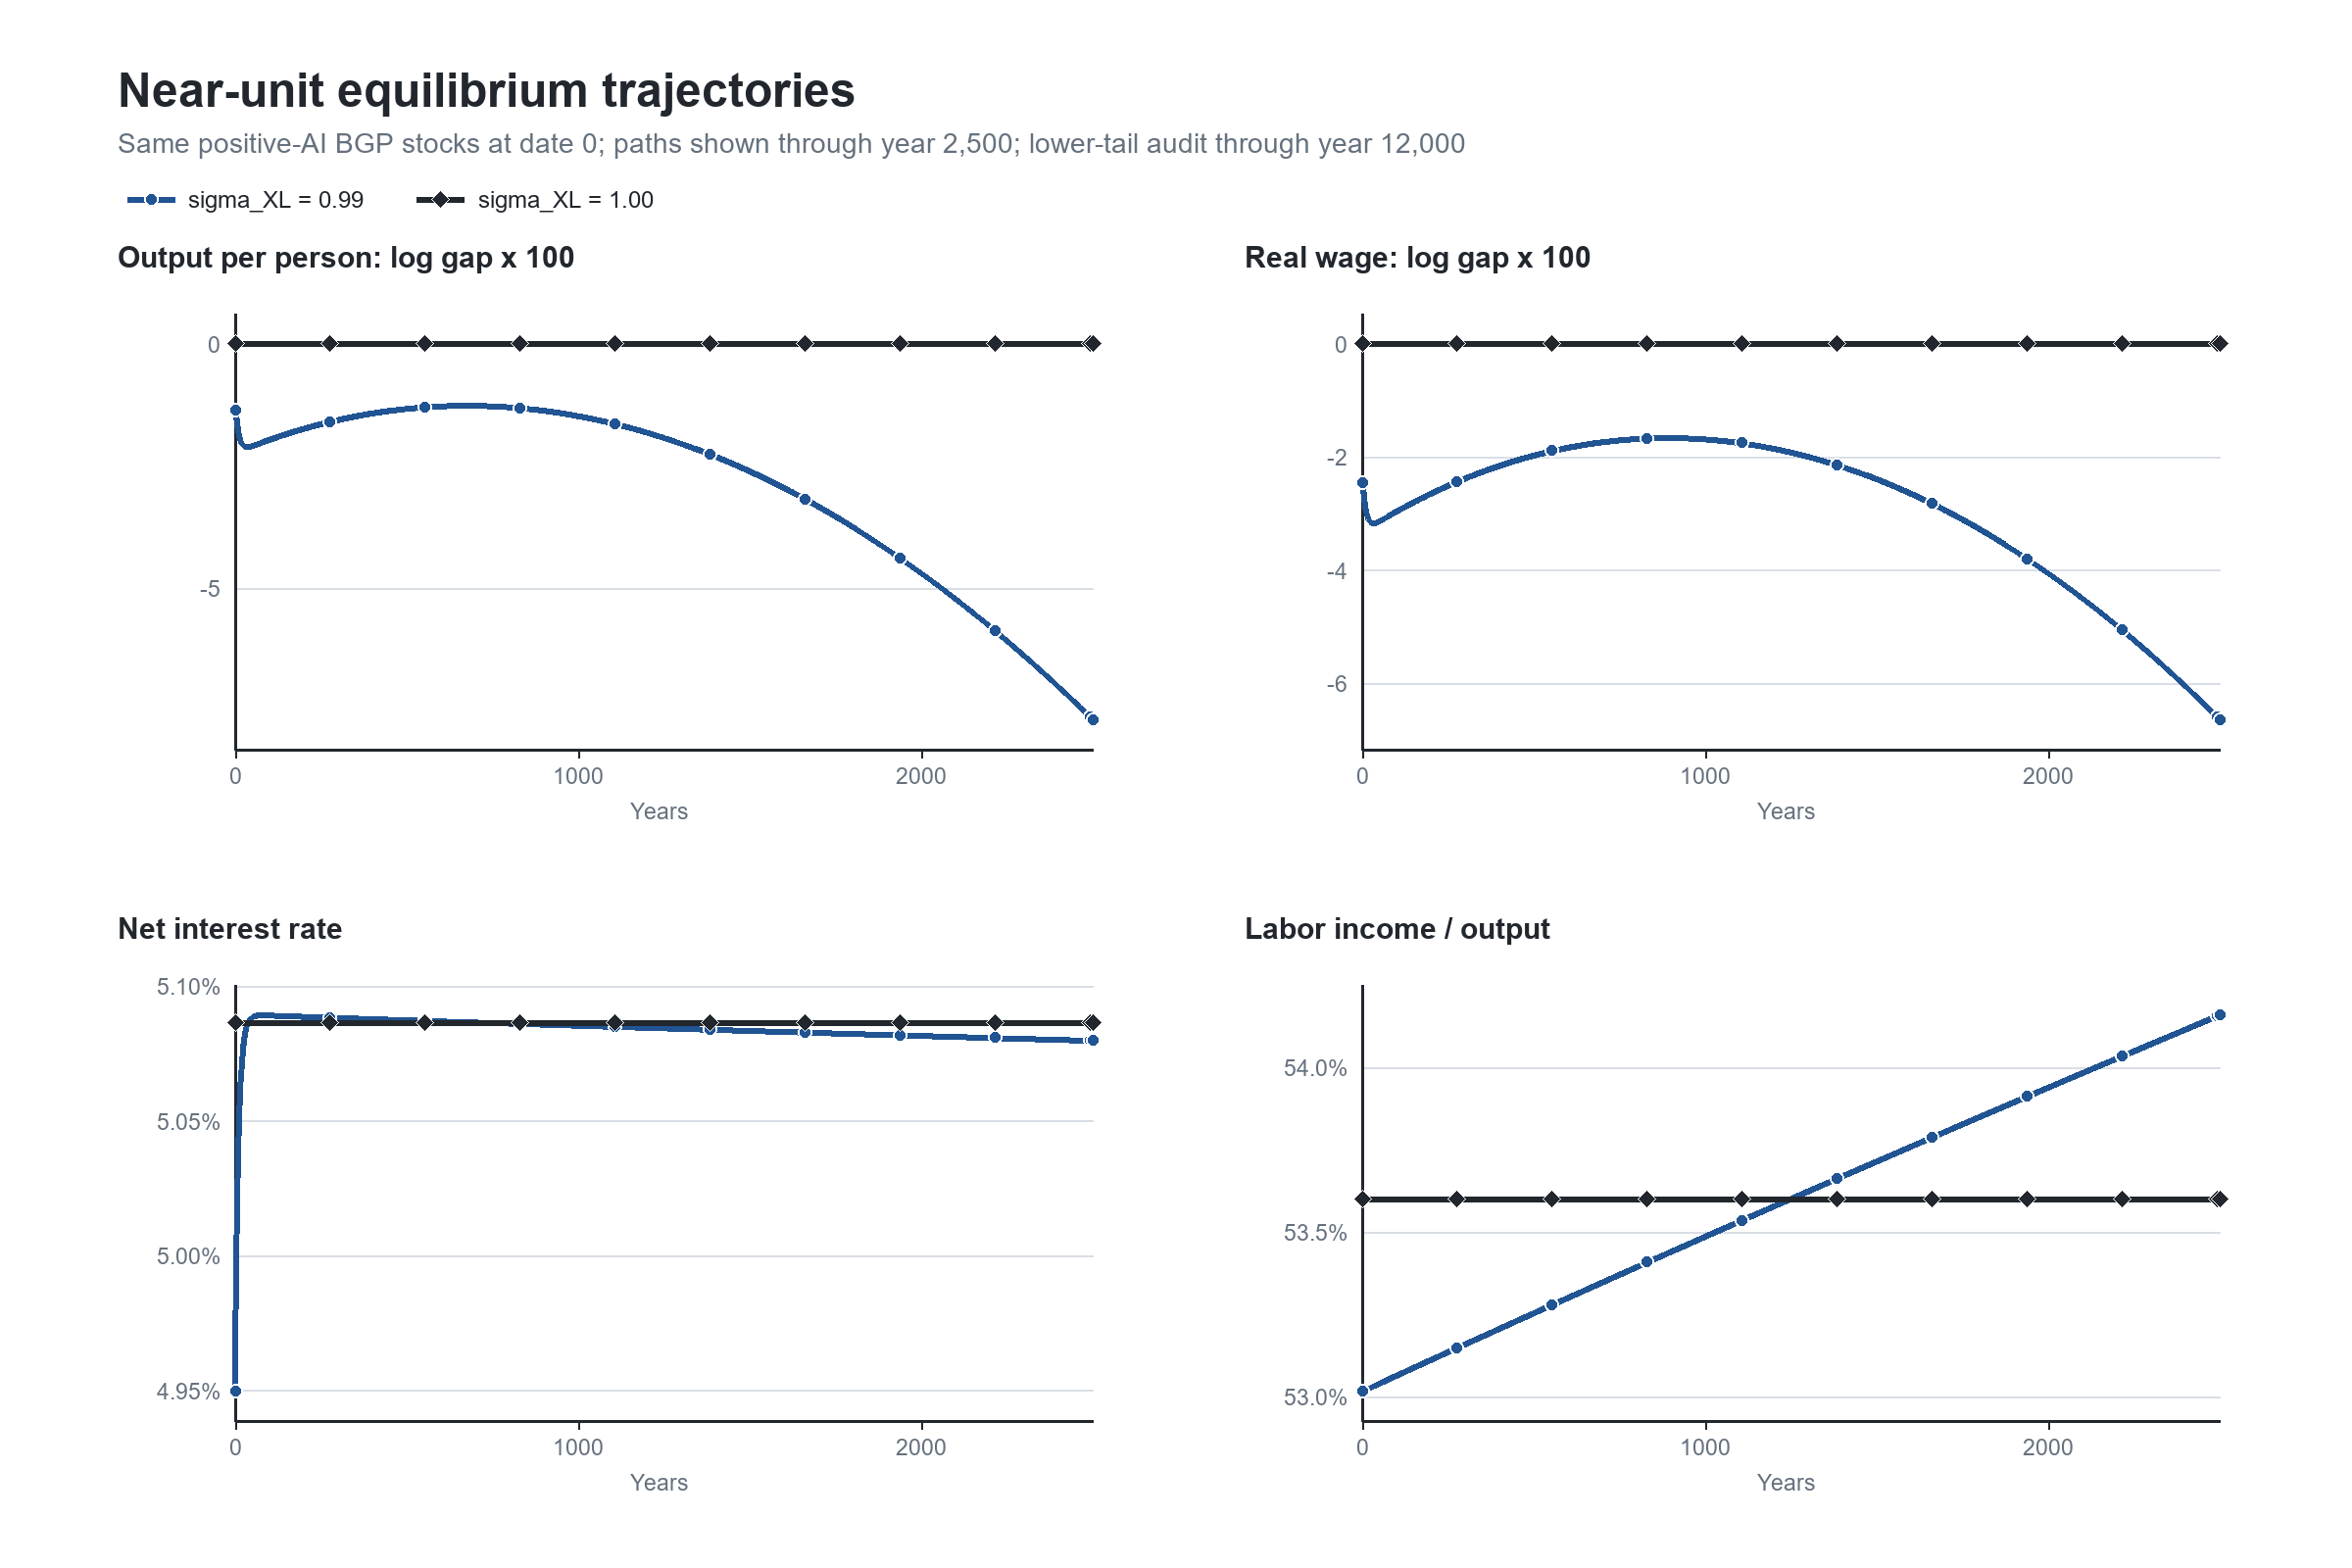
\includegraphics[width=\textwidth]{figures_axm/axm_near_unit_equilibrium_paths.png}
\caption{Admitted near-unit equilibrium trajectories from common unit-elastic
balanced-growth stocks. In both cases \(\omega_X=0.20\). The
\(\sigma_{XL}=0.99\) terminal audit extends through year 12,000, but I show only
years 0--2,500. The output and wage panels report 100 times the log difference
from the \(\sigma_{XL}=1\) equilibrium; the other panels report annual
percentages. Appendix \ref{app:axm-near-unit-equilibrium-paths} describes the
regime-specific terminal and admission tests.}
\label{fig:axm-near-unit-equilibrium}
\end{figure}

The initial distributional response reflects the fact that the common starting
stocks imply \(X/(AL)<1\). Equation
\eqref{eq:axm-near-unit-share-expansion} implies that lowering
\(\sigma_{XL}\) initially raises \(s_X\) and lowers labor's income share. As
\(X/(AL)\) grows, this ordering reverses. By year 2,500, 100 times the log gaps
in output per person and the real wage are \(-7.68\) and \(-6.64\),
respectively. Labor receives 54.16 percent of output, compared with 53.60
percent at unit elasticity, while the net interest rate remains close to its
unit-elastic value.

This experiment documents one-sided finite-date continuity between two admitted
equilibria, not similarity of their long-run paths. For a fixed nonunit
elasticity,
\(h=\varphi\ln[X/(AL)]\) accumulates over time and eventually becomes
economically important. Thus the limits \(\sigma_{XL}\to1\) and
\(t\to\infty\) need not commute. The regime propositions, rather than this
finite-window comparison, characterize the conditional long-run regimes. A
bilateral equilibrium comparison around one remains incomplete until an
admissible \(\sigma_{XL}>1\) equilibrium is constructed. Proposition
\ref{prop:axm-no-regular-gross-substitutes-continuation} rejects both regular
continuations used by the algorithm, so the admission rule rejects the computed
finite-window path instead of presenting it as an equilibrium.

Finally, these are functional distribution results, not predictions about
interpersonal inequality. The representative household supplies all labor and
owns both physical capital and the developer. A vanishing labor-income share
also need not imply a falling real wage: along the conditional gross-substitutes
branch, the wage can rise while \(wN/Y\) falls because output grows faster than
labor income.

\subsection{Cross-regime synthesis and limits of the evidence}

The feedback mechanism differs across regimes. Complementarity keeps \(X/(AL)\)
finite because raw inference compute falls as capability rises. Unit elasticity
produces the constant limiting matrix \(\mathcal F(\bar s)\). Gross substitution
makes the feedback state dependent; on the conditional AI-dominated branch it is
summarized by \(\Omega_\infty\). These are distinct economic regimes rather than
small perturbations around Cobb--Douglas.

The propositions characterize limits under their stated hypotheses. The
reported simulations are restricted to the complementary-input and
unit-elasticity trajectories that pass the equilibrium-admission rule. The
gross-substitutes free-boundary calculation remains a diagnostic of a
conditional pre-singular solution of the necessary conditions; it is not
reported as an equilibrium trajectory and does not establish global optimality
or selection of that branch from arbitrary initial states.
